% Ersteller: 	Daniel Wirth
% Software:	TeX-Distribution --> MiKTeX (https://miktex.org/); Editor --> Texmaker (https://www.xm1math.net/texmaker/)
% Literatur:	.bib erstellt mit JabRef (https://www.jabref.org/); %Achtung: bilatex-mode verwenden (preferences) und dann .bib-file erstellen; Engine --> biber
% Der nachfolgende Praxisbericht wurde für das Praxisseminar im Studiengang BEI angefertigt.
%

\documentclass[a4paper, portrait, 12pt]{scrartcl} % Vorgabe TH Nbg
%%%%%%%%%%% Präambel %%%%%%%%%%%

% Standardpakete
%\usepackage[latin1]{inputenc}
\usepackage[T1]{fontenc}
\usepackage[ngerman]{babel}
\usepackage[left=3cm, right=2cm]{geometry} % Vorgabe TH Nbg
\usepackage{graphicx}
\graphicspath{ {../../img/} }
\usepackage{amsmath,amsfonts}
\usepackage{siunitx}
\usepackage{textcomp} % €
\usepackage[dvipsnames]{xcolor}
\usepackage{xspace} % Sorgt dafür, dass Leerzeichen hinter parameterlosen Makros nicht als Makroendezeichen interpretiert werden

% Formatierung etc.: Allgemein
\usepackage{setspace}
\onehalfspacing % Vorgabe TH Nbg
%\spacing{1.X}
\setlength{\parindent}{0pt} % Kein Einzug
\usepackage{afterpage}
\usepackage{lastpage}
\usepackage{fancyhdr} % Für beliebige Kopf- und Fußzeilen
\pagestyle{fancy}
\fancyhf{} % Löscht vorherige Einstellungen - Gesamt
%\fancyhead{} % Löscht voherige Einstellungen
%\fancyfoot{} % Dito
\renewcommand{\headrulewidth}{0 pt} % Keine obere Trennlinie
%\(this)pagestyle{empty} % Keine Seitenzahlen
%\setcounter{page}{n} % Bestimme Seite mit n bezeichnen, nachfolgende ist dann n+1
\rfoot{\thepage\ von \pageref{LastPage}} % Seite x von y; Vorgabe TH Nbg
\usepackage{enumitem}


% Formatierung etc.: Schrift
\usepackage{lmodern} % bessere Fonts
%\usepackage{ulem} % Unterstreichen
\usepackage{relsize} % Schriftgröße relativ festlegen


% Formatierung etc.: Tabellen/Arrays
%\usepackage{tabularx} % "Einfacher Tabllen gestalten"
%\usepackage{adjustbox}
\usepackage{caption} % Beschriftung von Bildern/Tabellen
\usepackage{subcaption} % Analog zu oben
%\setlength{\topsep}{0pt} % Kein xtra Abstand über Tabulator	
%\setlength{\partopsep}{0pt} % Kein xtra Abstand unter Tabulator	

% Code-Snippets
\usepackage{listings}

% Hyperlinks und URLs etc.
\usepackage[ 
       colorlinks=true,		%% wenn keine Farbigen Links: = false
    ]{hyperref}
\hypersetup{colorlinks=true, linkcolor=black, urlcolor=MidnightBlue, citecolor=black}
\urlstyle{same}


% Graphiken, Plots, PDFs etc.
%!TEX root = name.tex % Andere .tex-Datei einbinden
\usepackage{pdfpages}
\usepackage{float}
\usepackage{wrapfig}
%\usepackage{pgfplots}
%\pgfplotsset{width=10cm,compat=1.9} % Zweiten Parameter nicht verändern!


% Rechtschreibung bzw. Trennung
%\hyphenchar\font=\string"7F % Nötig für korrekte Silbentrennung!
%\hyphenation{Kom-pli-ziert-es-Wort}
%\hyphenpenalty = XXX
%\tolerance = XXX


% Mathe
%\usepackage{aligned-overset}
%\usepackage{mathabx} %\widehat{•} & \widecheck{}


% "Speziellere" Befehle
%\newcommand{\forceindent}{\leavevmode{\parindent=1.5em\indent}}


% Bibliographie
\usepackage[style=alphabetic, backend=biber]{biblatex}  
\usepackage{csquotes} % Für Anführungszeichen bei Zitaten
\addbibresource{Bibliographie_Projekt_USB_Oszi.bib}
%\usepackage[nohyperlinks, printonlyused]{acronym} % Abkürzungsverzeichnis


% define style for code snippets
\definecolor{codegreen}{rgb}{0,0.6,0}
\definecolor{codegray}{rgb}{0.5,0.5,0.5}
\definecolor{codepurple}{rgb}{0.58,0,0.82}
\definecolor{codefunc}{rgb}{0,0.3,0.7}
\definecolor{backcolour}{rgb}{0.95,0.95,0.92}

\lstdefinestyle{mystyle}{
    backgroundcolor=\color{backcolour},   
    commentstyle=\color{codegreen},
    keywordstyle=\color{magenta},
    identifierstyle=\color{codefunc},
    numberstyle=\tiny\color{codegray},
    stringstyle=\color{codepurple},
    basicstyle=\ttfamily\footnotesize,
    breakatwhitespace=false,         
    breaklines=true,                 
    captionpos=b,                    
    keepspaces=true,                 
    numbers=left,                    
    numbersep=5pt,                  
    showspaces=false,                
    showstringspaces=false,
    showtabs=false,                  
    tabsize=2
}

\lstset{style=mystyle}

\title{Projekt USB-Oszilloskop}
\author{Samuel Oeser, Nicole Sturm, Daniel Wirth}
\date{\today}


%%%%%%%%%%% Main %%%%%%%%%%%
\begin{document}

\setlist{noitemsep}	% no item separation in lists

%%%%%%%%%%% Deckblatt %%%%%%%%%%%
\maketitle
%\thispagestyle{empty}
\pagebreak

%%%%%%%%%%% TOC %%%%%%%%%%%
%\thispagestyle{empty}
\tableofcontents
\pagebreak

%%%%%%%%%%% Abstract / Zusammenfassung %%%%%%%%%%%
\section{Abstract / Zusammenfassung}

\pagebreak

%%%%%%%%%%% Einleitung %%%%%%%%%%%
\section{Einleitung}
Die vorliegende Projektarbeit wurde im Rahmen des Bachelorstudiengangs Elektrotechnik und Informationstechnik an der Fakultät für Elektrotechnik, Feinwerktechnik und Informationstechnik (EFI) der Technischen Hochschule Nürnberg Georg Simon Ohm durchgeführt. Ziel des Projekt-Moduls ist es, den Studierenden die Möglichkeit zu geben, ihr theoretisch erworbenes Wissen in einem praxisnahen, ingenieurwissenschaftlich strukturierten Entwicklungsprojekt anzuwenden. Die Motivation für die Auswahl des Projektthemas lag in der Abbildung des vollständigen Entwicklungsprozesses eines aus Hardware, Firmware und Software bestehenden Gesamtsystems. Auf diese Weise konnten praxisnahe Erfahrungen in allen wesentlichen Entwicklungsdisziplinen gesammelt werden. Darüber hinaus bot das Projekt die Gelegenheit, die grundlegenden Funktionen eines Oszilloskops zu verstehen und im Rahmen eines Prototyps zu realisieren. Ein weiteres wesentliches Auswahlkriterium für das Thema war die klare Unterteilung in abgegrenzte Aufgabenbereiche, sodass die Teammitglieder ihre Aufgaben eigenständig bearbeiten konnten, während gleichzeitig eine Zusammenarbeit im übergeordneten Kontext möglich war.\\

Das zu Beginn definierte Ziel des Projekts war die Entwicklung eines USB-Oszilloskops. Das Gesamtsystem, bestehend aus selbstentwickelter Hardware und einem über Universal Serial Bus (USB) angeschlossenen Computer, soll die Grundfunktionen eines digitalen Speicheroszilloskops (DSO) abbilden. Die Realisierung sollte durch den Einsatz eines Analog-Digital-Umsetzers (ADC) zur Messwerterfassung sowie eines Mikrocontrollers ($\mu$C) als Schnittstelle zwischen der Hardware (ADC-Schaltung) und der Software (Computer) erfolgen.\\

Das Projektteam setzte sich aus drei Studierenden zusammen: Samuel Oeser war verantwortlich für die Entwicklung der Hardware (HW), Daniel Wirth übernahm die Firmware (FW), während Nicole Sturm die Software (SW) einschließlich der grafischen Benutzeroberfläche (GUI) entwickelte. Die Betreuung des Projekts erfolgte durch Prof. Dr. Sven Loquai, der die Studierenden während des gesamten Entwicklungsprozesses begleitete.
\pagebreak

%%%%%%%%%%% Fachliche Grundlagen %%%%%%%%%%%
\section{Fachliche Grundlagen}

\subsection{Allgemeiner Aufbau eines DSOs}
\label{subsec:oscilloscope_func}
Das DSO erfasst Eingangssignale, digitalisiert sie und stellt die Messdaten nach Speicherung und Verarbeitung dar. Der grundlegende Aufbau umfasst die Eingangsumschaltung (DC AC GND) mit Vertikalverstärkung/abschwächung, den ADU mit Signalvorverarbeitung, den Datenspeicher, Takt und Steuerung, die Triggereinrichtung sowie die Anzeige. Die digitalisierten Daten werden im Speicher abgelegt und für Darstellung und Auswertung ausgelesen (vgl. \cite[S. 216]{Muehl2020}).

\begin{figure}[H]
	\centering
    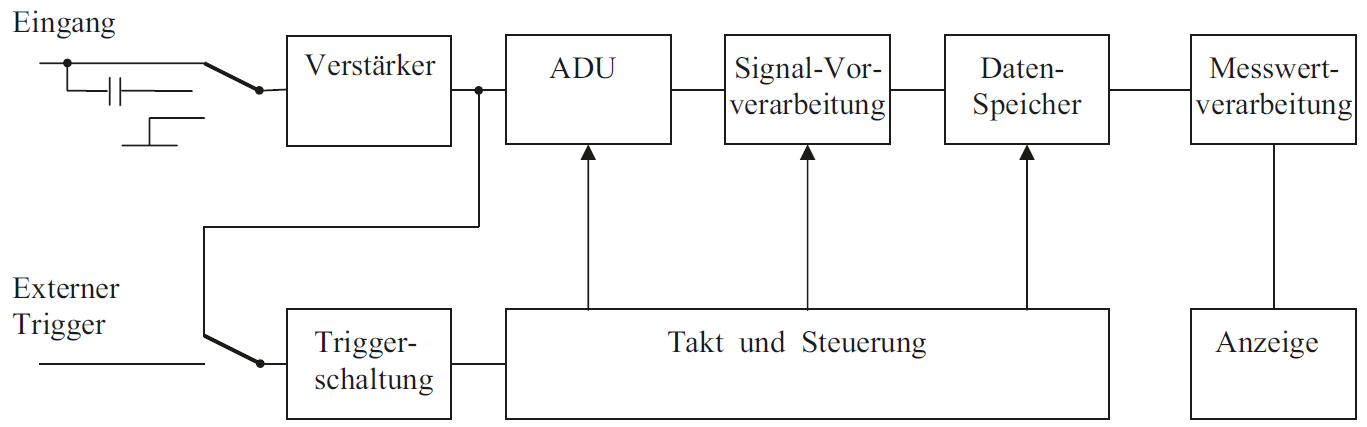
\includegraphics[scale=0.4]{block_diagram_oscilloscope_muehl.png} 
	\caption{Blockschaltbild eines Digitaloszilloskops (Abb. 14.1 aus \cite[S. 216]{Muehl2020})}
	\label{fig:blockdiagram_oscilloscope}
\end{figure}

Für die Abtastung sind zwei Betriebsarten relevant. Die Echtzeitabtastung erfasst den kompletten Verlauf in einem Durchlauf und die zeitliche Auflösung wird durch die Rate des AD-Umsetzers (ADU) begrenzt. Die Äquivalenzzeitabtastung rekonstruiert sehr schnelle periodische Verläufe aus mehreren Durchläufen (vgl. \cite[S. 216]{Muehl2020}).

\begin{figure}[H]
	\centering
    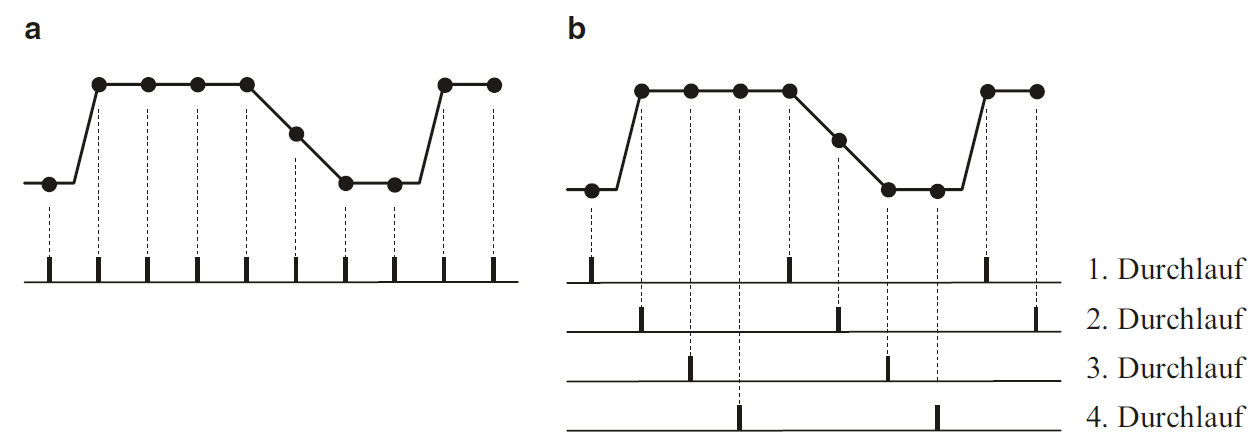
\includegraphics[scale=0.4]{real_equivalent_sampling_muehl.png} 
	\caption{Gegenüberstellung Echtzeitabtastung (a) und Äquivalenzzeitabtastung (b) (Abb. 14.2 aus \cite[S. 216]{Muehl2020})}
	\label{fig:real_equivalent_sampling}
\end{figure}

Für eine gut auswertbare Darstellung sind etwa zehn Stützstellen je Periode zweckmäßig und die si-Interpolation (auch sinc-Interpolation genannt) ermöglicht bei erfüllter Nyquist Bedingung eine nahezu verzerrungsfreie Rekonstruktion. In der Praxis sollte die maximale Signalfrequenz mindestens um den Faktor 2,5 unter der Abtastrate liegen (vgl. \cite[S. 218f]{Muehl2020}).

\begin{figure}[H]
	\centering
		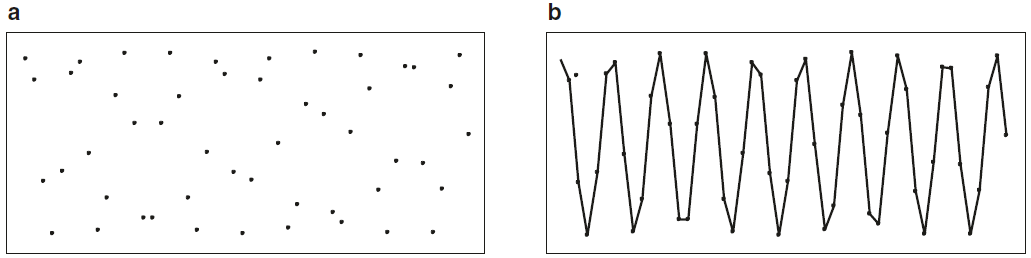
\includegraphics[scale=0.4]{point_linear_display_muehl.png} 
		\caption{\centering Punktedarstellung (a) und lineare Interpolation (b)\\(Abb. 14.4 aus \cite[S. 218]{Muehl2020})}
	\label{fig:point_linear_display}
\end{figure}

\begin{figure}[H]
	\centering
		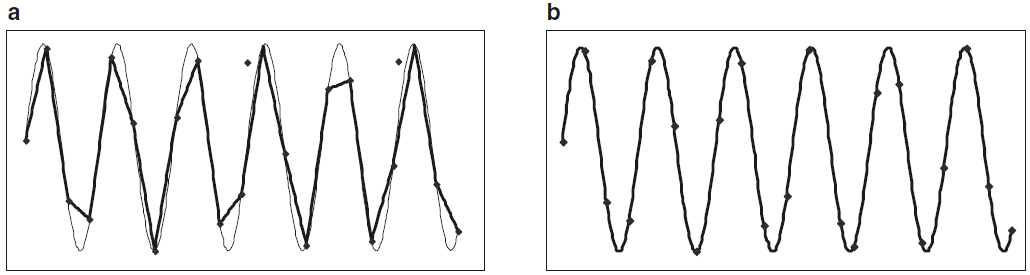
\includegraphics[scale=0.4]{linear_si_display_muehl.png} 
		\caption{\centering Lineare Interpolation (a) und si-Interpolation (b)\\(Abb. 14.5 aus \cite[S. 219]{Muehl2020})}
	\label{fig:linear_si_display}
\end{figure}

In der Praxis werden für die Digitalisierung schnelle Flash-ADUs sowie mehrstufige Sub-ranging- / Pipeline‑Varianten eingesetzt. Diese ermöglichen hohe Raten bei moderater vertikaler Auflösung. Übliche Geräte arbeiten mit acht Bit vertikaler Auflösung. Je nach Architektur sind höhere Auflösungen möglich (vgl. \cite[S. 114-119]{Bernstein2023}). Für die Datenaufnahme stehen verschiedene Acquisition-Modi zur Verfügung. Der direkte Modus liefert äquidistante Samples. Min-Max oder Peak-Detect erfasst Extremwerte innerhalb eines Abtastintervalls und macht kurze Spikes sichtbar. Average reduziert Rauschen durch wiederholtes Mitteln. Single Shot zeichnet einmalige Ereignisse auf und der Roll-Modus zeigt sehr langsame Verläufe kontinuierlich an (vgl. \cite[S. 220f]{Muehl2020}). Die Genauigkeit wird wesentlich durch die Abtastrate und Abtaststrategie, Interpolation und Quantisierung sowie durch die Eingangsbeschaltung bestimmt. Bei Unterabtastung droht Aliasing und die Rekonstruktion wird unzuverlässig (vgl. \cite[S. ??]{Muehl2020}, Grundlagen zur Abtastung und Quantisierung). Wichtige Kenngrößen DSOs sind analoge Bandbreite, Abtastrate, vertikale Auflösung, Speichertiefe, Triggerfunktionen, Eingangsimpedanz, analoge Eingangsspannung sowie Anzeige und Darstellungsoptionen. Über die Kurvendarstellung hinaus gehören auch automatische Messfunktionen zum Grundumfang.

\subsubsection{Trigger}

Die Triggerung steuert die Signalspeicherung. Fortlaufend erfasste Abtastwerte laufen in einen Ringspeicher und beim Triggerereignis wird das Überschreiben gestoppt, sodass Pre Trigger und Post Trigger gezielt darstellbar sind (vgl. \cite[S. 216f]{Muehl2020}).

\begin{figure}[H]
	\centering
		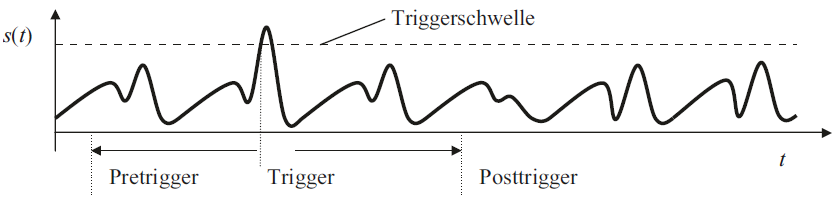
\includegraphics[scale=0.5]{trigger_oscilloscope_muehl.png} 
		\caption{\centering Messsignal $s(t)$ mit eingestellter Triggerschwelle und Triggerzeitpunkt\\(Teilabbildung der Abb. 14.3 aus \cite[S. 217]{Muehl2020})}
	\label{fig:trigger_oscilloscope}
\end{figure}

Die analoge Triggerkette umfasst Quelle, Kopplung DC oder AC, einstellbare Triggerschwelle, Flankenrichtung, Hysterese und Auto Trigger. Sie erzeugt ein robustes Triggersignal für die Speichersteuerung (vgl. \cite[S. 210-212]{Muehl2020}).

\begin{figure}[H]
	\centering
		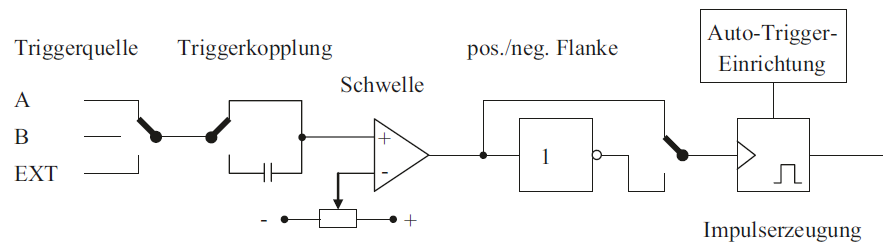
\includegraphics[scale=0.5]{trigger_circuit_oscilloscope_muehl.png} 
		\caption{\centering Funktionsblöcke einer Triggereinrichtung (Abb. 13.8 aus \cite[S. 212]{Muehl2020})}
	\label{fig:trigger_circuit_oscilloscope}
\end{figure}

\subsubsection{Frequenzkompensierter Tastkopf / Spannungsteiler}

In der Praxis existieren verschiedene Arten von Tastköpfen wie passive, aktive und differenzielle Tastköpfe. Im Folgenden wird ausschließlich der frequenzkompensierte passive Tastkopf betrachtet, da er für das Projekt relevant ist (vgl. \cite[Kap. 15]{Muehl2020}). Dieser Tastkopf basiert auf einem frequenzkompensierten Spannungsteiler (seihe \autoref{fig:freq_compensated_vdiv}), realisiert als RC Teiler mit zu den Widerständen parallel geschalteten Kapazitäten und mit einer Anpassung an die Summe aus Bauteil- und Leitungskapazitäten. Die Kompensation mit Trimmkondensator (in \autoref{fig:freq_compensated_vdiv}: $C_T$) wird so abgeglichen, dass das Teilungsverhältnis im Nutz-Frequenzband annähernd konstant bleibt. Der Abgleich erfolgt mit einem Rechtecksignal. Unterkompensation zeigt sich durch eine nach unten geneigte Oberkante (\autoref{fig:freq_compensated_time}a), Überkompensation durch eine nach oben geneigte Oberkante (\autoref{fig:freq_compensated_time}c) und bei korrekter Kompensation bleibt die Oberkante über die Pulsbreite hinweg horizontal (\autoref{fig:freq_compensated_time}b) (vgl. \cite[S. 104-106]{Schruefer2022}).

\begin{figure}[H]
	\centering
		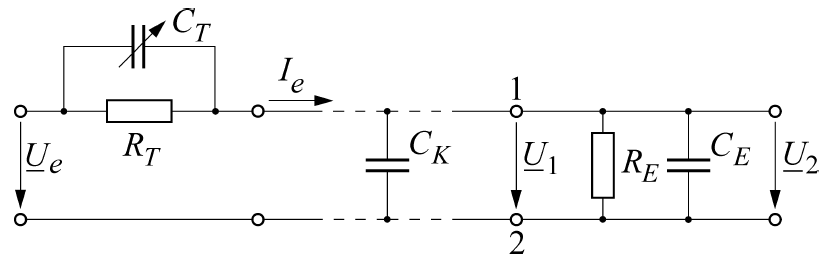
\includegraphics[scale=0.5]{freq_compensated_vdiv_schruefer.png} 
		\caption{\centering Tastteiler am Eingang eines Oszilloskops (Bild 2.42 aus \cite[S. 105]{Schruefer2022})}
	\label{fig:freq_compensated_vdiv}
\end{figure}

\begin{figure}[H]
	\centering
		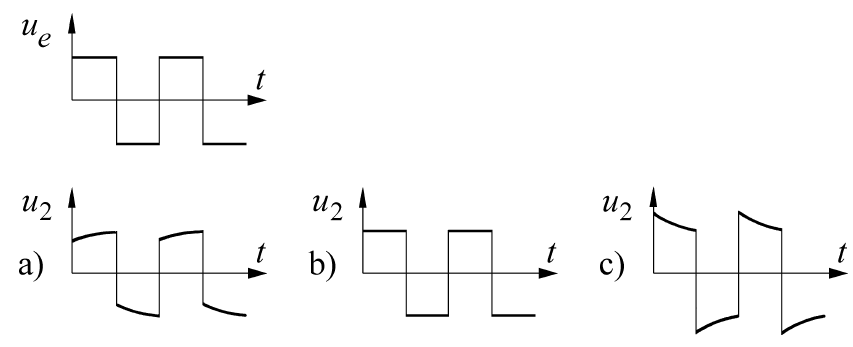
\includegraphics[scale=0.5]{freq_compensated_time_schruefer.png} 
		\caption{\centering Rechteckimpulse an RC-Spannungsteiler (Bild 2.43 aus \cite[S. 106]{Schruefer2022})\\ \footnotesize (a) unterkompensiert, (b) richtig kompensiert, (c) überkompensiert}
	\label{fig:freq_compensated_time}
\end{figure}


Mit $R_1=R_T$ und $C_1=C_T$ gilt für die obere Teilimpedanz ($\underline{Z_1}$):
\begin{equation}
	\underline{Z_1}=R_1||\frac{1}{j\omega C_1}=\frac{R_1}{1+j\omega R_1 C_1}
	\label{eq:z1}
\end{equation}
und mit $R_2=R_E$ und $C_2=C_K+C_E$ gilt für die untere Teilimpedanz ($\underline{Z_2}$):
\begin{equation}
	\underline{Z_2}=R_2||\frac{1}{j\omega C_2}=\frac{R_2}{1+j\omega R_2 C_2}
	\label{eq:z2}
\end{equation}
Über den Spannungsteiler ergibt sich aus (\ref{eq:z1}) und (\ref{eq:z2}) das Verhältnis:
\begin{equation}
	\frac{\underline{U_1}}{\underline{U_2}}=\frac{\underline{Z_1}+\underline{Z_2}}{\underline{Z_2}}=1+\frac{\underline{Z_1}}{\underline{Z_2}}=1+\frac{R_1}{R_2}\frac{1+j\omega R_2 C_2}{1+j\omega R_1 C_1}
	\label{eq:comp_vdiv}
\end{equation}
Dieses Verhältnis nimmt den frequenzunabhängigen Wert $\frac{\underline{U_1}}{\underline{U_2}}=1+\frac{R_1}{R_2}$ an, wenn gilt:
\begin{equation}
	R_1\cdot C_1=R_2\cdot C_2
\end{equation}
Durch Einsetzen der Einzelbauelemente für $R_1$, $R_2$, $C_1$ und $C_2$ und Auflösen nach $C_T$ ergibt sich für den Trimmkondensator ein Wert nach \autoref{eq:ct_compensated_vdiv}, damit der Spannungsteiler frequenzunabhängig wird (vgl. \cite[S. 104-106]{Schruefer2022}).

\begin{equation}
	C_T=\frac{R_E\cdot (C_K+C_E)}{R_T}
	\label{eq:ct_compensated_vdiv}
\end{equation}

\subsection{AAF-Entwurf (Nyquisttheorem)}
\label{subsec:aaf_nyquist}

Ein Digitaloszilloskop erfasst das analoge Eingangssignal durch Abtastung mit einer bestimmten Frequenz. Diese Abtastung entspricht der Multiplikation des Signals mit einer Reihe von Impulsen, was im Frequenzbereich einer Faltung entspricht. Eine eindeutige Rekonstruktion aus den Abtastwerten setzt ein bandbegrenztes Eingangssignal mit höchster relevanter Frequenz und eine Abtastrate oberhalb des Doppelten dieser Frequenz voraus. Bei Unterschreitung falten sich Spektralkopien in das Basisband zurück und erzeugen Aliasse. Dies wird im Frequenzbild durch die Überlappung periodischer Spektren sichtbar in \autoref{fig:aaf_freq_domain} sowie im Zeitbereich durch scheinbar niedrigere Schwingungen in \autoref{fig:aliasing_time_domain}. Aus dieser Grundlage folgt die Notwendigkeit eines vorgeschalteten Anti-Aliasing-Tiefpasses, der außerbandige Anteile vor der Wandlung ausreichend dämpft (vgl. \cite[S. 314-316]{Bernstein2023} und \cite[S. 151-156]{Bernstein2024}).

\begin{figure}[H]
	\centering
		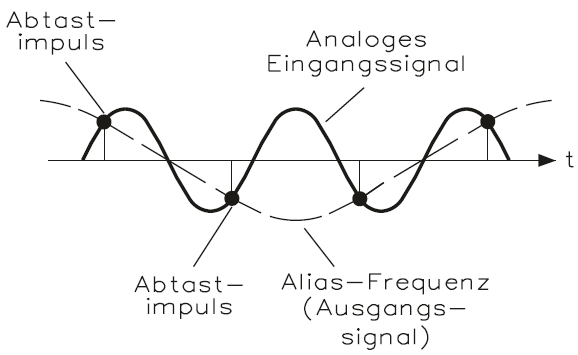
\includegraphics[scale=0.5]{aliasing_time_domain_bernstein.png} 
		\caption{\centering Aliasing: Erzeugung einer Scheinfrequenz durch unpassende Abtastrate\\ (Bild 2.71 aus \cite[S. 154]{Bernstein2024})
		}
	\label{fig:aliasing_time_domain}
\end{figure}

\begin{figure}[H]
	\centering
		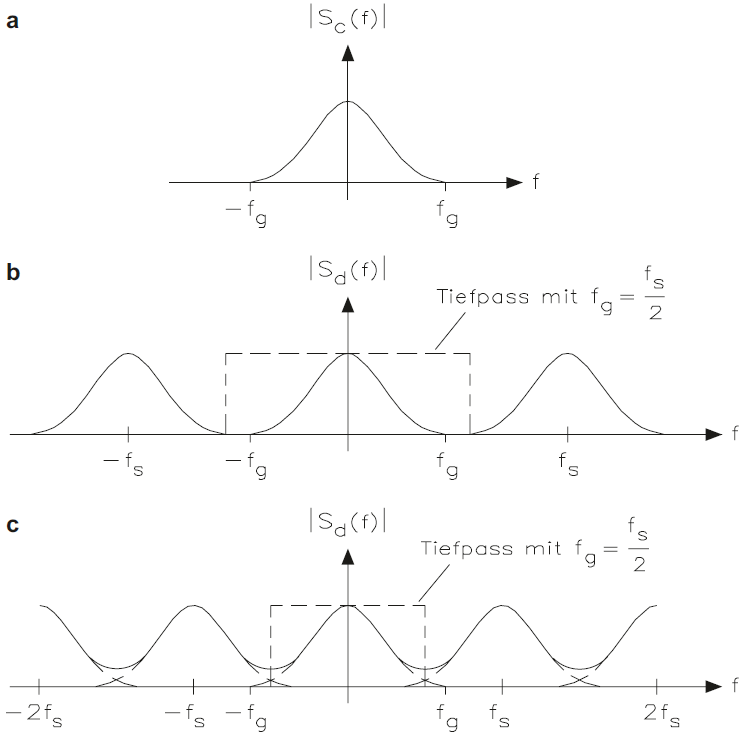
\includegraphics[scale=0.5]{aaf_freq_domain_bernstein.png} 
		\caption{\centering Abtasttheorem (Bild 4.30 aus \cite[S. 314]{Bernstein2023})\\
			\footnotesize(a) Betragsspektrum des bandbegrenzten Signals\\
			(b) Vervielfachung des Basisspektrums durch Abtastung mit $f_S > 2\cdot f_g$\\
			(c) Aliasing infolge zu niedriger Abtastrate ($f_S < 2\cdot f_g$)
		}
	\label{fig:aaf_freq_domain}
\end{figure}

Da der Entwurf des Anti-Aliasing-Filters maßgeblich durch den ausgewählten AD-Umsetzer bestimmt wird, sollte dieser zuerst festgelegt werden. Für aktive RC-Filter bewährt sich wegen Bauteiltoleranzen und des nicht idealen Übergangs vom Durchlass- in den Sperrbereich eine Abtastrate oberhalb der Mindestbedingung, typischerweise etwa 2.5 bis 4 mal $f_{max}$ und bei strengen Dämpfungszielen, z.B. wegen höheren Auflösungen, auch 5 bis 10 mal $f_{max}$. Eine höhere Abtastrate erweitert zudem die Übergangsbreite und senkt damit die notwendige Filterordnung, erleichtert die direkte Darstellung des abgetasteten Signals ohne Rekonstruktionsalgorithmen und erlaubt eine Filterfamilie mit geringerer Gruppenlaufzeitvariation und damit besserem Zeitverhalten. Aus der gewählten Abtastrate folgt dann die Nyquist-Frequenz $f_N = \frac{f_S}{2}$ und die Übergangsbreite $\Delta f = f_N - f_{max}$ \cite{Pini2020}.\\

Der theoretische, aus der Auflösung abgeleitete Dynamikbereich setzt eine Obergrenze für die sinnvoll anzustrebende Sperrbanddämpfung. Für einen \emph{N}-Bit-Umsetzer mit Full-Scale-Range \emph{FSR} gilt die Codebreite $Q = \frac{FSR}{2^N}$. Ein voll ausgesteuertes Störsignal soll auf einen Pegel unterhalb der Codebreite gedämpft werden, damit keine signifikanten Quantisierungsartefakte entstehen. Die Sperrbanddämpfung, beginnend an der Nyquist-Frequenz, wird daher so festgelegt, dass aliasingverursachende Anteile unterhalb der Codebreite bleiben:

\begin{equation}
	A(f_N)_{max}=20\cdot log_{10}\left( \frac{FSR}{Q}\right) =20\cdot log_{10}(2^N)=6.02\cdot N\hspace{0.1cm}dB
\end{equation}

In der Praxis begrenzt das $SINAD$ häufig den nutzbaren Dynamikbereich des gewählten AD-Umsetzers. Gilt $|SINAD|<|A_{max}|$ oder liegt die daraus ermittelte $ENOB$ (siehe \autoref{subsubsec:adc_characteristics} ``\nameref{subsubsec:adc_characteristics}``) unter der Auflösung des ADCs, dominieren Rauschen- und Verzerrungen. Bei Einsatz einer Mittelwertbildung kann es dennoch zweckmäßig sein, die Obergrenze $A_{max}$ anzusetzen. Im Regelfall wird die Sperrbanddämpfung an der Nyquistfrequenz so gewählt, dass gilt (vgl. \cite{Pini2020}):

\begin{equation}
	A(f_N)\approx min(|A_{max}|, |SINAD_{ADC}|)
\end{equation}

Die Bewertung des entworfenen Filters erfolgt in einem Tool wie dem Analog Filter Wizard über die Diagramme von Amplitudengang, Phasen- und Gruppenlaufzeit sowie Sprung- und Impulsantwort. Der Frequenzgang belegt Passband-Flachheit, Übergangsbreite und die Dämpfung an $f_N$. Phase und Gruppenlaufzeit zeigen, ob das Filter im Nutzband annähernd eine konstante Verzögerung liefert und damit Impulse und Flanken formtreu bleiben. Die Sprungantwort offenbart Überschwinger und Einschwingzeit. Eine Toleranzanalyse der zu erwartenden Widerstands- und Kapazitätsstreuungen zeigt, ob die Reserven ausreichend dimensioniert wurden (vgl. \cite{Pini2020} und \cite{Padmanabhuni2017}).

\subsection{Analog-to-Digital-Converter (ADC)}
\label{subsec:adc}

Ein Digitaloszilloskop benötigt einen AD-Umsetzer als zentrales Hardwareelement, da erst die Wandlung des analogen Eingangssignals in digitale Messwerte die weitere Speicherung, Verarbeitung und Anzeige ermöglicht. Für die Auswahl steht die Topologie am Anfang, weil sie Abtastrate, erreichbare Auflösung, Latenz, Leistungsaufnahme und den Implementierungsaufwand bestimmt.\\

Für ein USB-Oszilloskop bieten sich Flash- und Pipeline-Topologien an, da beide hohe Abtastraten für breitbandige Zeitbereichsmessungen bereitstellen. Andere Varianten wie SAR oder Delta-Sigma werden in den Quellen überwiegend mittleren Geschwindigkeiten oder schmalbandigen Präzisionsaufgaben zugeordnet und sind somit für ein USB-Oszilloskop irrelevant (vgl. \cite{MPS} und \cite{AnalogDevices2001a}).\\

\subsubsection{Flash-ADC}
\autoref{fig:2bit_flash_adc} zeigt das Prinzip eines Flash-AD-Umsetzers mit zwei Bit. Eine Widerstandsleiter erzeugt abgestufte Referenzen und eine Komparatorbank vergleicht das Eingangssignal mit diesen Schwellen. Das resultierende Muster wird durch eine Logikschaltung in einen Binärcode überführt. Flash-ADCs erreichen, durch diesen simplen Aufbau, die höchste Geschwindigkeit. Da die Zahl der Komparatoren jedoch $2^N-1$ beträgt, steigen bei hohen Auflösungen Komplexität, Fläche, Leistungsaufnahme sowie insbesondere die Herstellungskosten annähernd exponentiell an (vgl. \cite{MPS} und \cite{AnalogDevices2001b}).

\begin{figure}[H]
	\centering
		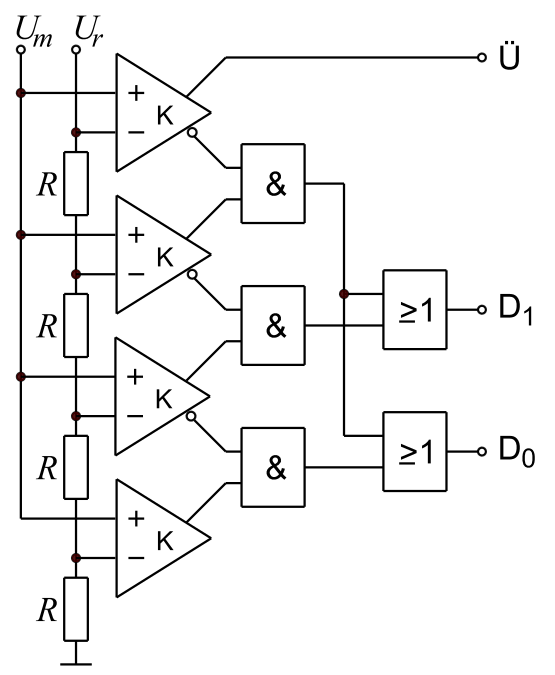
\includegraphics[scale=0.3]{DMT_ADU-2-Bit-Flash.png} 
		\caption{\centering  Flash-Umsetzer mit 2 Bit, einschl. Kodeumsetzer\\
		\footnotesize Ersteller: Saure, Quelle: \href{https://de.wikipedia.org/wiki/Datei:DMT_ADU-2-Bit-Flash.svg}{[Link]} (Lizenz: \href{https://creativecommons.org/licenses/by-sa/3.0/}{CC BY-SA 3.0})
		}
	\label{fig:2bit_flash_adc}
\end{figure}

\subsubsection{Pipeline-ADC}
Eine Alternative zur geringeren Skalierbarkeit des Flash-ADCs ist der Pipeline-ADC, der auch im Projekt zur Anwendung kommt. Er baut funktional auf dem Flash-Prinzip auf, indem mehrere niedrigauflösende Flash-ADCs in Stufen hintereinandergeschaltet werden. Am Eingang tastet eine Sample-and-Hold-Stufe das Signal ab. Jede Stufe wandelt in wenige Bits, rekonstruiert den quantisierten Anteil über einen DAC, bildet den Restfehler im Subtrahierer und verstärkt diesen für die nächste Stufe. Durch Überlappbits und digitale Fehlerkorrektur können die Genauigkeitsanforderungen an die einzelnen Stufen reduziert werden und die Durchsatzraten erhöht. Durch diesen Aufbau steigt der Aufwand mit zunehmender Auslösung nur linear an. Bauartbedingt entsteht allerdings eine definierte Zykluslatenz, die in ganzen oder halben Taktzyklen angegeben wird. Diese Latenz ist der entscheidende Nachteil eines Pipeline ADCs (vgl. \cite{MPS} und \cite{AnalogDevices2001c}).

\begin{figure}[H]
	\centering
		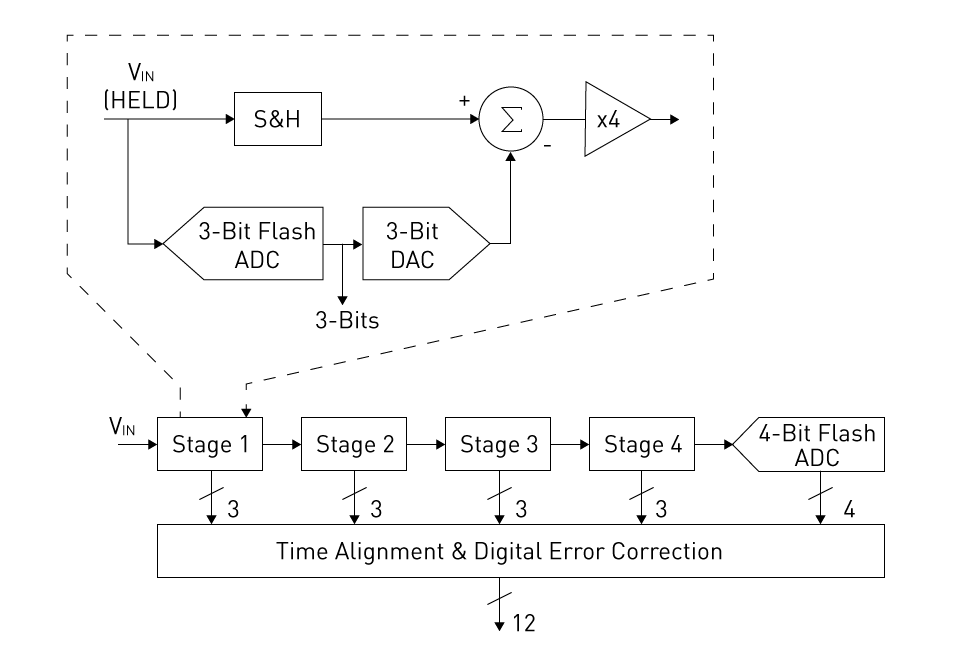
\includegraphics[scale=0.3]{ADC_Chapter_2_Fig4-_960_x_658.png} 
		\caption{\centering 12-bit pipelined ADC\\ \footnotesize Ersteller: MPS, Quelle: \href{https://www.monolithicpower.com/en/learning/mpscholar/analog-to-digital-converters/detailed-analysis-of-adc-architectures/pipeline-adcs}{[Link]} (Ch. 2, Fig. 4)
		}
	\label{fig:pipelined_adc}
\end{figure}
\pagebreak

\subsubsection{Wichtige Kenngrößen von AD-Umsetzern}
\label{subsubsec:adc_characteristics}

Die Kenngrößen und deren Definition können dem IEEE Standard 1241-2023 \emph{``Terminology and Test Methods for Analog-to-Digital Converters``} (\cite[S. 22ff]{IEEE2023}) entnommen werden.\\

\textbf{Auflösung und Eingangsbereich}\\
Die Auflösung eines \emph{N}-Bit-AD-Umsetzers umfasst $2^N$ binäre Codes. Der differentielle Eingangspannungssbereich wird als Full-Scale Range (\emph{FSR}) bezeichnet und in Volt angegeben. Das LSB entspricht $\frac{FSR}{2^N}$.\\

\textbf{Maximale Sampling-Rate}\\
Die Abtastrate ist der Kehrwert der Abtastperiode (Abstand zwischen Abtastwerten). Sie bestimmt die zeitliche Auflösung und ist insbesondere in Bezug auf das Niyqusttheorem relevant.\\

\textbf{Leistungsaufnahme}\\
Die Leistungsaufnahme ist in erster Linie für die Auslegung der Versorgungsspannung und der zugehörigen Leitungen relevant.\\

\textbf{Verstärkungsfehler}\\
Der Verstärkungsfehler beschreibt die Abweichung der Kennliniensteigung von der idealen Steigung nach Offsetkorrektur und wird in $LSB$ oder in Prozent der Full-Scale-Range angegeben.\\

\textbf{Offsetfehler}\\
Der Offsetfehler ist die vertikale Verschiebung der Kennlinie relativ zur Referenzgeraden und wird in $LSB$ oder in Prozent der Full-Scale-Range angegeben.\\

\textbf{Latenz}\\
Die Latenz wird als Pipeline-Delay in ganzen oder halben Taktzyklen angegeben oder alternativ als Zeitangabe und beschreibt den Abstand zwischen Abtastung und Verfügbarkeit des zugehörigen Digitalworts.\\

\textbf{Differentielle Nichtlinearität $DNL$}\\
Die DNL ist die Abweichung der tatsächlichen Codebreite $W[k]$ von der idealen Codebreite $Q$, normiert auf $Q$, und wird in $LSB$ angegeben. Die Codebreite entspricht dem Spannungsbereich, der dem Code zugeordnet ist. Formal gilt $DNL[k]=\frac{W[k]}{Q}-1$.\\
Die Angabe im Datenblatt entspricht $max\hspace{0.1cm}DNL[k]$.\\

\textbf{Integrale Nichtlinearität $INL$}\\
Abweichung des Übergangsspannungsniveaus von einem Code in den nächsten zu dem der idealisierten Geraden, nach Korrektur von Offset und Verstärkung.\\
Damit gilt $INL[k]=\sum_{n=0}^kDNL[n]$. Die Angabe im Datenblatt entspricht $max\hspace{0.1cm}INL[k]$.\\

\textbf{Rausch- und Verzerrungsmaße}\\
\textbf{$SNR$} gibt das Verhältnis von Nutzsignal- zu Rauschleistung an:
\begin{equation}
	SNR_{dB}=10\cdot \log_{10}\left( \frac{P_{Signal}}{P_{Rauschen}}\right)
\end{equation}

\textbf{$THD$} ist ein Maß für das Verhältnis von harmonischen Verzerrungen zur Grundschwingung:
\begin{equation}
	THD_{dB}=10\cdot \log_{10}\left( \frac{P_{Harmonische}}{P_{Signal}}\right)
\end{equation}

\textbf{$SINAD$} umfasst harmonische Verzerrungen und Rauschen:
\begin{equation}
	SINAD_{dB}=10\cdot \log_{10}\left( \frac{P_{Signal}}{P_{Rauschen}+P_{Harmonische}}\right)
\end{equation}

\textbf{$ENOB$} ist die effektive Bitzahl und wird aus SINAD abgeleitet:
\begin{equation}
	ENOB\approx \frac{SINAD[dB]-1.76}{6.02}
\end{equation}





\pagebreak

\subsection{Endliche Zustandsautomaten (Finite State-Machines - FSMs)}
\label{subsec:fsm}
Die Firmware und Software des Projekts sind als synchronisierte Zustandsautomaten implementiert, um einen deterministischen Ablauf der beiden Programme zu gewährleisten.
\subsubsection{Definition und formale Darstellung}
Ein endlicher Automat (EA - engl. Finite State Machine, FSM) ist ein abstraktes Rechenmodell zur Beschreibung von Systemen. Dieser befindet sich in mindestens einem Zustand von einer Zahl endlicher Zustände. Zustandsübergänge (sog. Transitionen) erfolgen durch Eingaben oder das Auftreten von Ereignissen (spezielle Form der Eingabe).\\

Zustände modellieren, was das System gerade tut bzw. in welchem internen ``Modus`` es sich befindet. Ereignisse sorgen für den Wechsel zwischen Zuständen. Übergänge definieren, wie das System im aktuellen Zustand auf ein Ereignis reagiert.

Ein FSM besteht nach \cite[S. 7ff]{Baesig2019} typischerweise aus:
\begin{itemize}
	\item einer Menge von Zuständen $S$,
	\item einem Anfangszustand $s_0$,
	\item einem Eingabe- oder Ereignisalphabet $E$ (Events),
	\item einem Ausgabealphabet $A$,
	\item einer Zustandsübergangsfunktion $\delta :S\times E\rightarrow S$,
	\item einer Ausgabefunktion $\lambda :S\times E\rightarrow A$,
	\item und einer endlichen (evtl. leeren) Menge der Endzustände $F$.
\end{itemize}

Je nach Modellierung kann das Ausgabealphabet und die Ausgabefunktion, sowie die Menge an Endzuständen entfallen.\\

Unterschieden werden folgende Arten von Endlichen Automaten:
\begin{itemize}
	\item \emph{Deterministische Endliche Automaten (DEA)}:\\
	Ein Automat wird als deterministisch bezeichnet, wenn für jede Kombination aus Eingabedaten und aktuellem Zustand eindeutig festgelegt ist, welcher Folgezustand erreicht wird. Das bedeutet, dass sich das \emph{System zu einem bestimmten Zeitpunkt stets in genau einem definierten Zustand} befindet.
	\item \emph{Nichtdeterministische Endliche Automaten (NEA)}:\\
	Bei einem NEA sind für einen bestimmten Zustand und eine Eingabe keine, genau ein oder mehrere mögliche Zustandsübergänge definiert.
\end{itemize}

DEAs sind einfacher als NEAs zu implementieren, wodurch diese in der Praxis häufiger zur Anwendung kommen (vgl. \cite[S. 14]{Baesig2019}). Im Projekt sind die FSMs als DEAs ausgeführt .\\

Eine weitere Aufgliederung von DEAs erfolgt nach der Abhängigkeit der Ausgabe, wenn diese vorhanden ist (vgl. \cite[S. 8f]{Baesig2019}).
\begin{itemize}
	\item Wenn die Ausgabe nur vom aktuellen Zustand abhängt, handelt es sich um einen \emph{Moore-Automaten}.
	\item Wenn die Ausgabe vom aktuellen Zustand \underline{und} der Eingabe abhängt, handelt es sich um einen \emph{Mealy-Automaten}.
\end{itemize}
Im Projekt kommen Moore-Automaten zur Anwendung.

\subsubsection{Modellierung und Darstellung}

Die Darstellung eines Zustandsautomaten erfolgt üblicherweise mit einem \emph{Zustandsdiagramm} (auch Zustandsübergangsdiagramm), einem gerichteten Graph\footnote{ ``Graphen sind ein [...] Konzept, um Objekte und die Beziehung zwischen diesen darzustellen.``\\Quelle: \href{https://www.tu-chemnitz.de/informatik/theoretische-informatik/TI-1/lecture-notes/06-00-graphs.html}{[Link]}}. Die Knoten stellen die Zustände der Menge $S$ dar und die gerichteten Kanten die Zustandsübergänge. Der Startzustand und die Endzustände werden gesondert gekennzeichnet. Eine übliche Darstellung für einen einfachen Moore-Automaten findet sich in \autoref{fig:statediagram_example}a (\emph{sn} sind die Zustände, \emph{xn} sind Eingaben oder Ereignisse und \emph{yn} sind Ausgaben; \emph{n = 1,2,...}) (vgl. \cite[S. 9]{Baesig2019}).\\

Die Darstellung des Zustandsdiagramms ist auch als Teil der \emph{Unified Modelling Language (UML)}\footnote{aktueller UML-Standard (V2.5.1): \href{https://www.omg.org/spec/UML/2.5.1/About-UML}{[Link]}} festgelegt, welche auch durch internationale Normung festgeschrieben ist. In der Praxis (vor allem beim händischen Entwurf von Zustandsdiagrammen) hat sich aber ein Mischform bewährt, welche auf einige Elemente der UML zurückgreift (siehe \autoref{fig:statediagram_example}b). Es lassen sich beispielsweise auch hierarchische Strukturen integrieren (verschachtelte Zustände).

\begin{figure}[H]
	\centering
    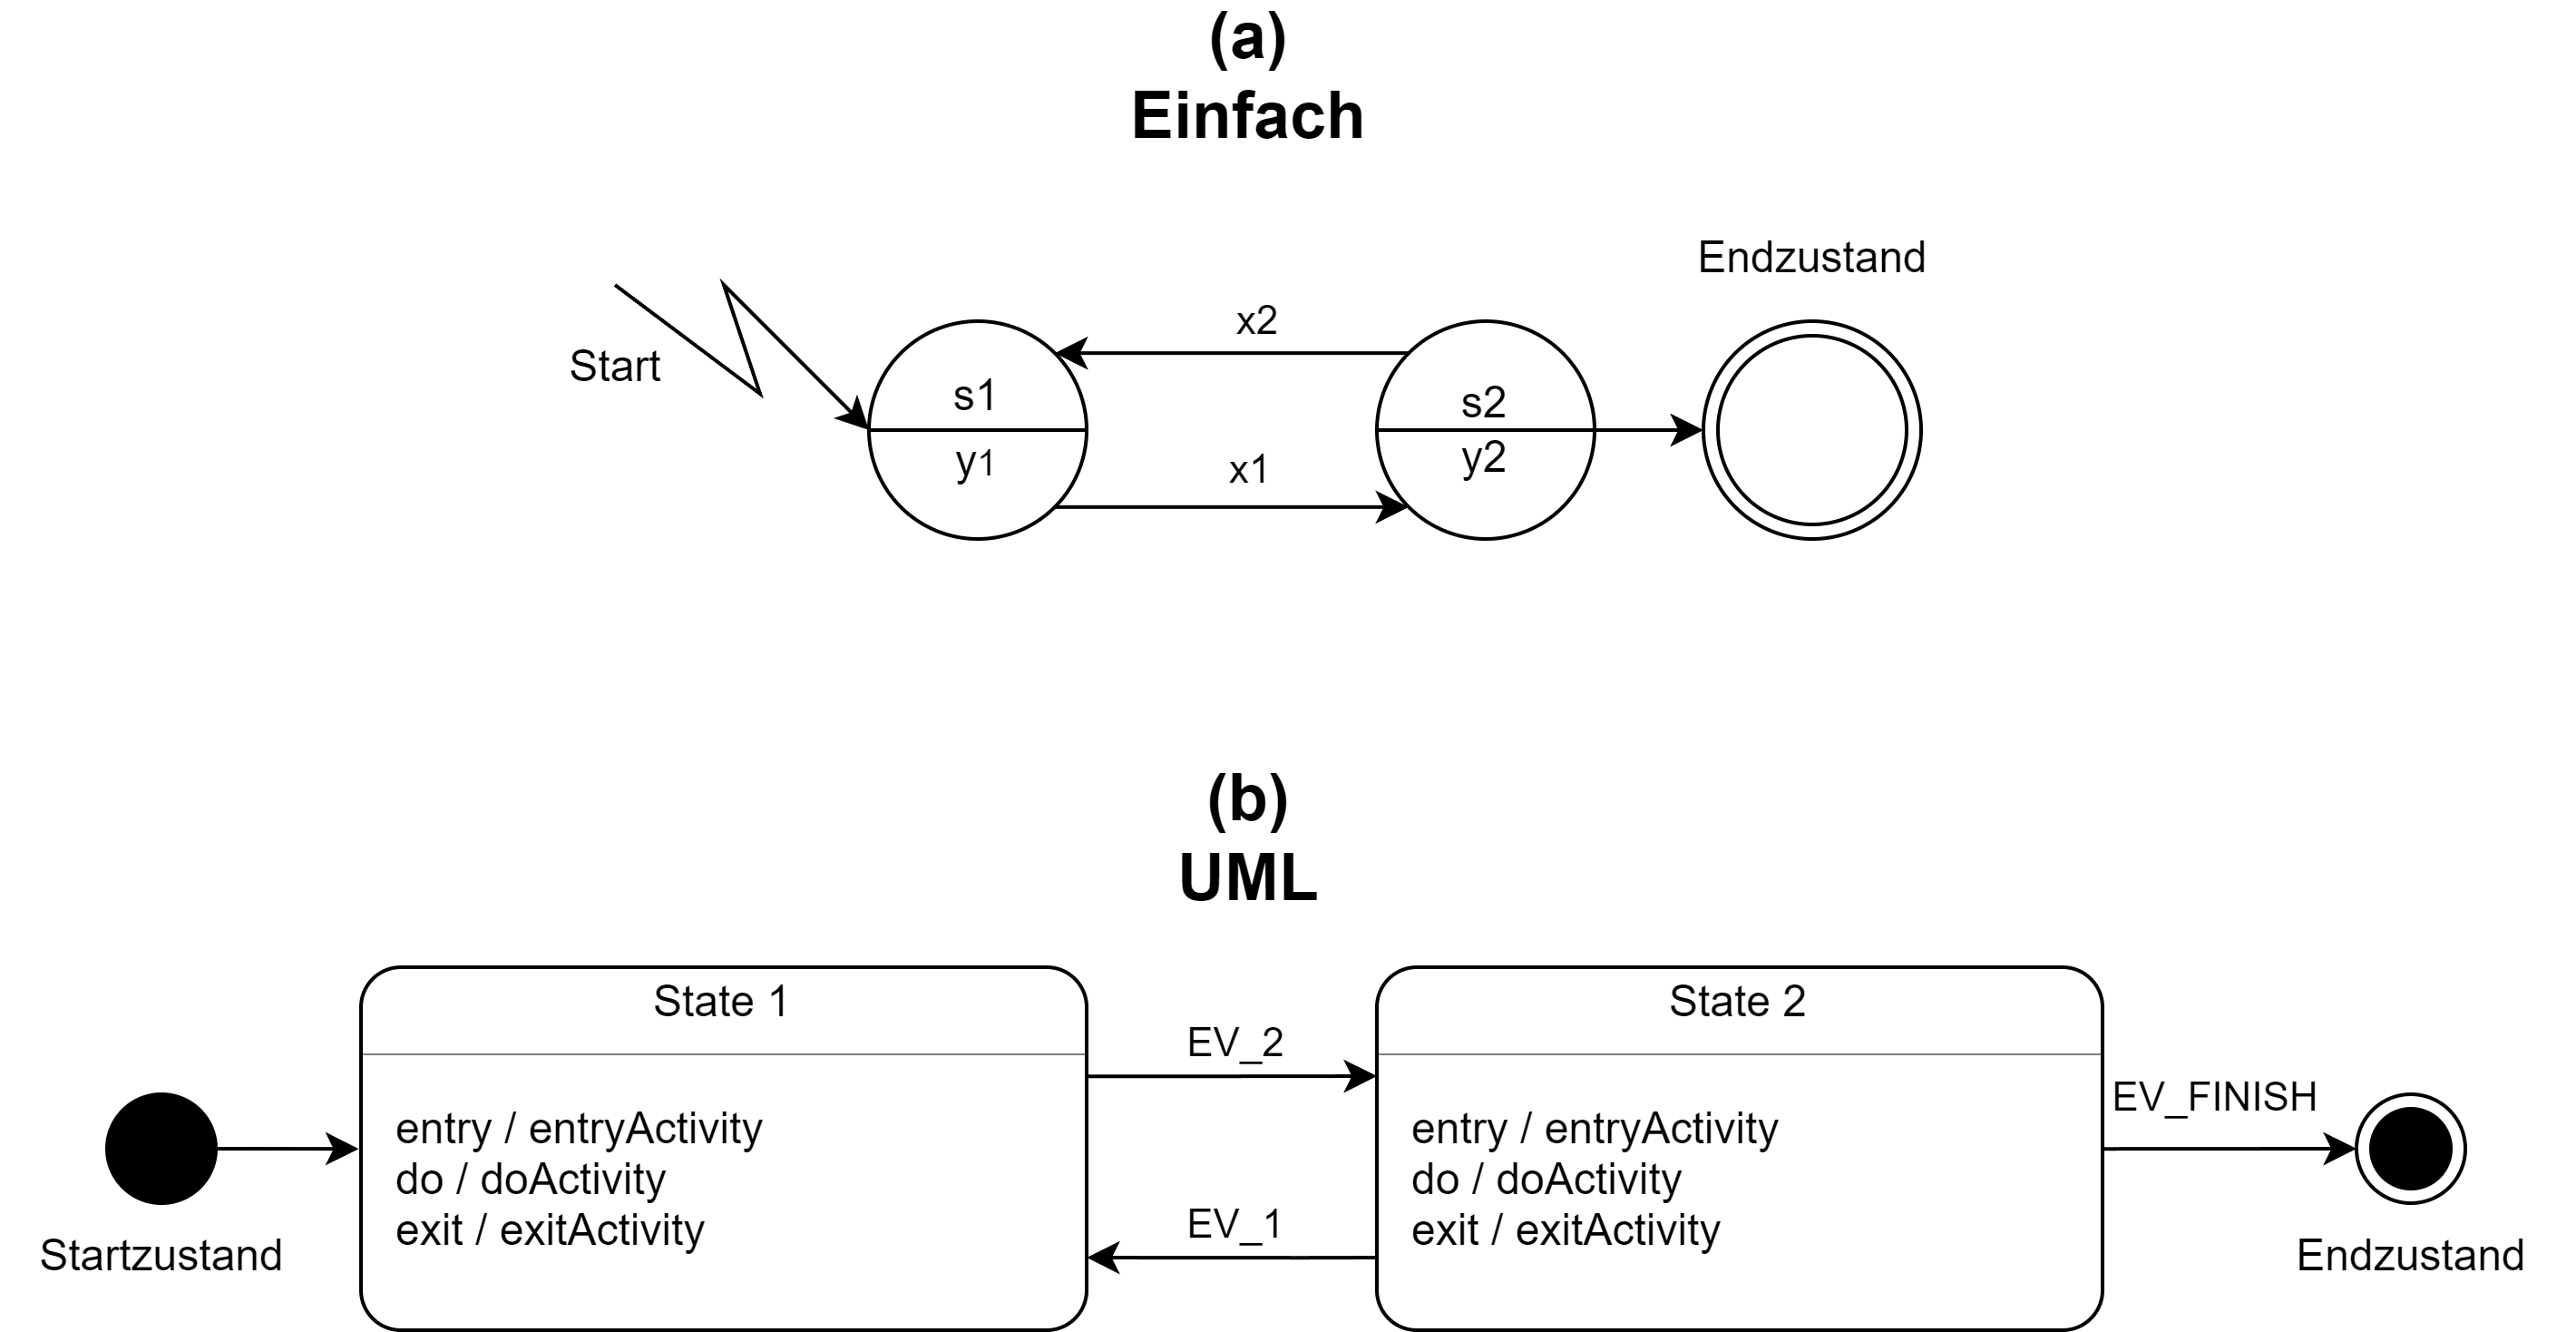
\includegraphics[scale=0.12]{StateDiagram_example.png} 
	\caption{(a) Zustandsdiagramm (nach \cite{Baesig2019}); (b) UML-Zustandsdiagramm}
	\label{fig:statediagram_example}
\end{figure}
\subsubsection{Vorteile einer FSM bei der Programmierung}
\begin{itemize}
	\item \emph{Klarheit \& Übersichtlichkeit}\\
	Der Systemverlauf ist in wohldefinierte Zustände gegliedert. Der Code wird hierdurch verständlicher (kein ``Spaghetti-Code``).
	\item \emph{Deterministisches Verhalten}\\
	Durch die Definitionen, wie auf welches Ereignis reagiert wird, kann die Vorhersagbarkeit und Zuverlässigkeit gewährleistet werden. Außerdem lassen sich undefinierte Zustände durch die explizite Modellierung vermeiden.
	\item \emph{Modularisierung \& Wiederverwendbarkeit}\\
	Einzelne Zustände oder Teile der FSM lassen sich kapseln, segmentieren und wiederverwenden. Teilbereiche können eventuell separat getestet werden.
	\item \emph{Wartbarkeit \& Erweiterbarkeit}\\
	Das System lässt sich durch Hinzufügen neuer Zustände oder neuer Übergänge modular erweitern, ohne die vorhandene Logik stark zu verändern.
	\item \emph{Kommunikation und Dokumentation}\\
	Zustandsdiagramme können bei der Vermittlung von komplexem Programmverhalten gegenüber Nicht-Programmieren genutzt werden.
	\item \emph{Verbessertes Debugging}\\
	Da Zustandsübergänge zentralisiert sind, lassen sich Log-Messages und weitere Debugging-Mechanismen leichter verwenden.
\end{itemize}

\subsection{Direct Memory Access - DMA}
\label{subsec:dma}
\subsubsection{Allgemeines}
DMA bezeichnet den Vorgang, bei dem durch eine dedizierte Einheit ohne Beteiligung einer CPU Daten transferiert werden (also als Hintergrundprozess). Er kommt zum Einsatz, wenn große Datenmengen von der Peripherie oder einem Speicher zu einem anderen transferiert werden müssen. Ein Chip oder eine Teileinheit eines Mikrocontroller (µC), die solche Transfers durchführt, heißt \emph{Direct Memory Access Controller (DMAC)} (vgl. \cite[S. 125]{Urbanek2020}). Im Folgenden soll die Funktionsweise anhand der Realisierung in der im Projekt verwendeten STM32-Mikrocontrollerfamilie erläutert werden.

\subsubsection{DMA bei STM32-Mikrocontrollern}
Der DMA-Controller ist ein AHB-Modul (AHB - advanced high-performance bus; standardisiertes Bussystem von ARM) und kann wie auch die CPU des µCs als Master auf diesen Bus (genauer auf die Bus-Matrix) zugreifen. Durch die Datentransfers, welcher der DMAC nach seiner Konfiguration ohne CPU-Beteiligung ermöglicht, kann die System-Performance deutlich erhöht werden. Die Datentransfers können hierbei per Software oder über angeschlossene Peripherieelemente über sog. \emph{Requests} gestartet werden. Wird als steuerndes Element beispielsweise ein Hardware-Timer genutzt ermöglicht dies die zeitlich exakte Taktung von Datentransfers \cite[S. 6]{STmicroelectronics2016}, was im Projekt für den Abtastvorgang genutzt wird.

Der µC besitzt zwei unabhängige DMAC (Aufbau siehe \autoref{fig:dmac}), deren Anbindung an Peripherie und Speicher unterschiedlich ausfällt, um alle Ressourcen des Systems flexibel zu verwenden.\\

Der DMAC besitzt 3 Schnittstellen:
\begin{itemize}
	\item \emph{slave port} zur Programmierung des DMAs
	\item \emph{2 master ports} \begin{itemize}
		\item \emph{peripheral port}: peripherieseitiger Datenanschluss
		\item \emph{memory port}: speicherseitiger Datenanschluss
	\end{itemize}
\end{itemize}

\begin{figure}[H]
	\centering
    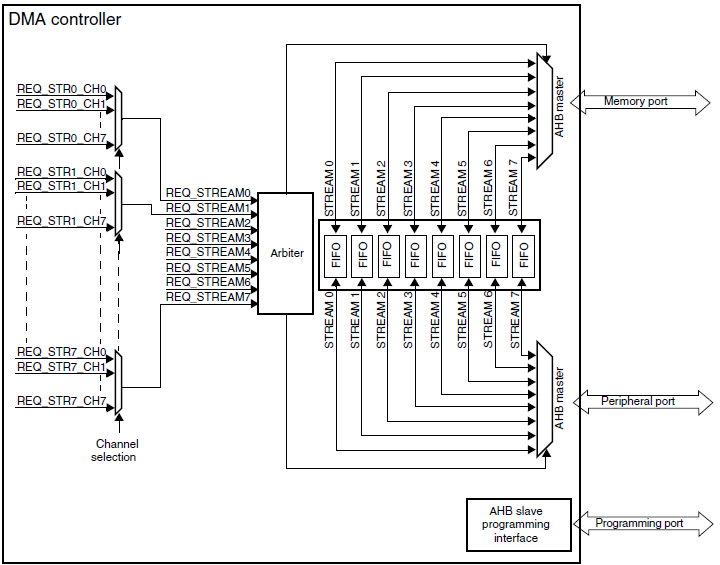
\includegraphics[scale=0.8]{STM32_DMAC.png} 
	\caption{Blockdiagramm STM32-DMA-Controller aus \cite[S. 7]{STmicroelectronics2016}}
	\label{fig:dmac}
\end{figure}

Jeder Controller besitzt 8 Datenwege (\emph{Streams}), die separat für unterschiedliche Datentransfers konfiguriert werden können (die Transfers können aber nicht gleichzeitig laufen). Die Streams besitzen hierbei eine konfigurierbare Priorität und ein zentrales Modul, der \emph{Arbiter}, regelt den Zugriff der Streams auf die Ports in Abhängigkeit der Priorität und sorgt für einen deterministischen Ablauf der Transfers. Die einzelnen Streams besitzen noch eine Anzahl an \emph{Channeln}, über die der entsprechende Peripherie-Request für einen Stream ausgewählt werden kann (vgl. \cite[S. 7ff]{STmicroelectronics2016}). Die Zuordnung eines Peripherie-Requests zu einer Channel-Stream-Kombination kann dem Reference-Manual des Controllers entnommen werden (für den STM32F767: \cite[S. 252]{STmicroelectronics2024}).

\pagebreak

Jeder Stream besitzt außerdem einen 4-stufige \emph{FIFO}-Pufferspeicher (First-In-First-Out), welcher Latenzen beim Zugriff auf das Übertragungsmedium (Bus-Switch-Matrix) überbrücken kann und ein \emph{Verpacken/Entpacken der Daten} erlaubt (z.B.: input: 8bit-Pakete, output: 32bit-Pakete; siehe \autoref{fig:dma_fifo}).

\begin{figure}[H]
	\centering
    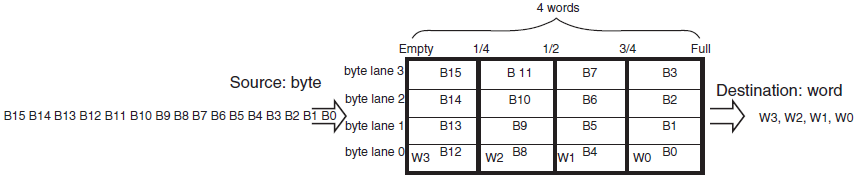
\includegraphics[scale=0.8]{STM32_DMA_FIFO.png} 
	\caption{FIFO-Struktur aus \cite[S. 11]{STmicroelectronics2016} (Teilabbildung)}
	\label{fig:dma_fifo}
\end{figure}

\textbf{\underline{DMA-Transfers}}\\
Ein Transfer wird zunächst über die \emph{Quelladresse (source address)} und \emph{Zieladresse (destination address)} charakterisiert, hier kann der DMA so konfiguriert werden, dass die Adressen nach einem Transfer automatisch inkrementiert werden können. Somit lassen sich, im Speicher hintereinanderliegende, Daten einfach übertragen. Quell- oder Zieladresse können jeweils aber auch konstant gehalten werden (siehe \autoref{fig:periph_to_mem}).

\begin{figure}[H]
	\centering
    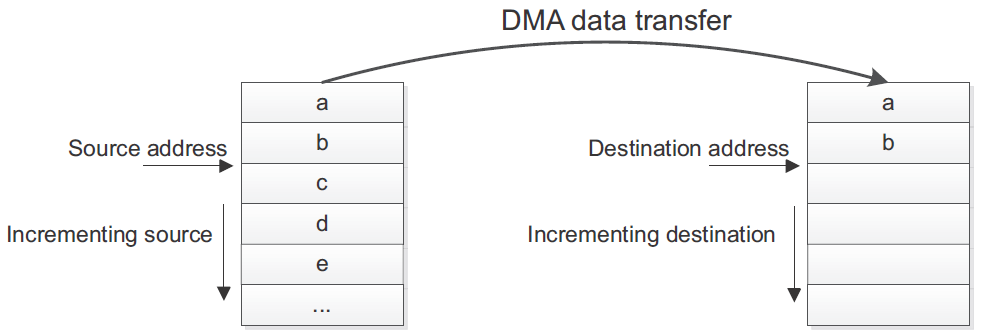
\includegraphics[scale=0.6]{STM32_DMA_transfer_incrementing.png} 
	\caption{DMA Quell- und Zieladressinkrementierung aus \cite[S. 10]{STmicroelectronics2016}}
	\label{fig:dma_transfer_inc}
\end{figure}

Weitere wichtige Parameter sind die Übertragungsgröße (transfer size), die in einem dedizierten Register (\emph{NDTR} - Number of Data Transfers Register) abgelegt ist, und die Datenbreite (Byte, Half-word, Word). Der Inhalt des NDTR wird nach jedem Transfer entsprechend der Größe des Transfers dekrementiert. Hier wird noch zwischen Circular mode und Normale mode unterschieden. Beim Normal mode ist eine Transaktion (bestehend aus NDTR Transfers) bei NDTR=0 beendet. Der Stream wird deaktiviert und es finden bis zum nächsten Aktivieren des Streams keine Transfers mehr statt. Beim Circular mode wird bei NDTR=0 das Register NDTR mit dem Initialwert geladen und die Transfers beginnen erneut (auch die Adressregister werden mit den Initialwerten geladen) $\rightarrow$ Kreislauf (circular).\\

Die drei möglichen Transfer-Modi sind:
\begin{itemize}
	\item Peripheral-to-Memory (siehe Beispiel in \autoref{fig:periph_to_mem}))
	\item Memory-to-Peripheral
	\item Memory-to-Memory
\end{itemize}

Bei einem Timer-Überlauf des Hardware-Timers TIM1 findet ein DMA-Request statt (ein Stream wurde hierbei entsprechend konfiguriert). Dieser Request löst einen Daten-Transfer zwischen Ziel und Quelle aus (die Datenbreite wurde im Beispiel auf 1 Byte festgelegt). Anschließend werden die Adressen entsprechend der Datenbreite inkrementiert, um die Ziel- und Quelladresse für den nächsten Transfer vorzubereiten. Dieser Prozess geschieht so lange, bis ``Number of Transfers`` durchgeführt worden sind. Der Wert von NDTR wird nach dem Transfer dekrementiert.\\

\begin{figure}[H]
	\centering
    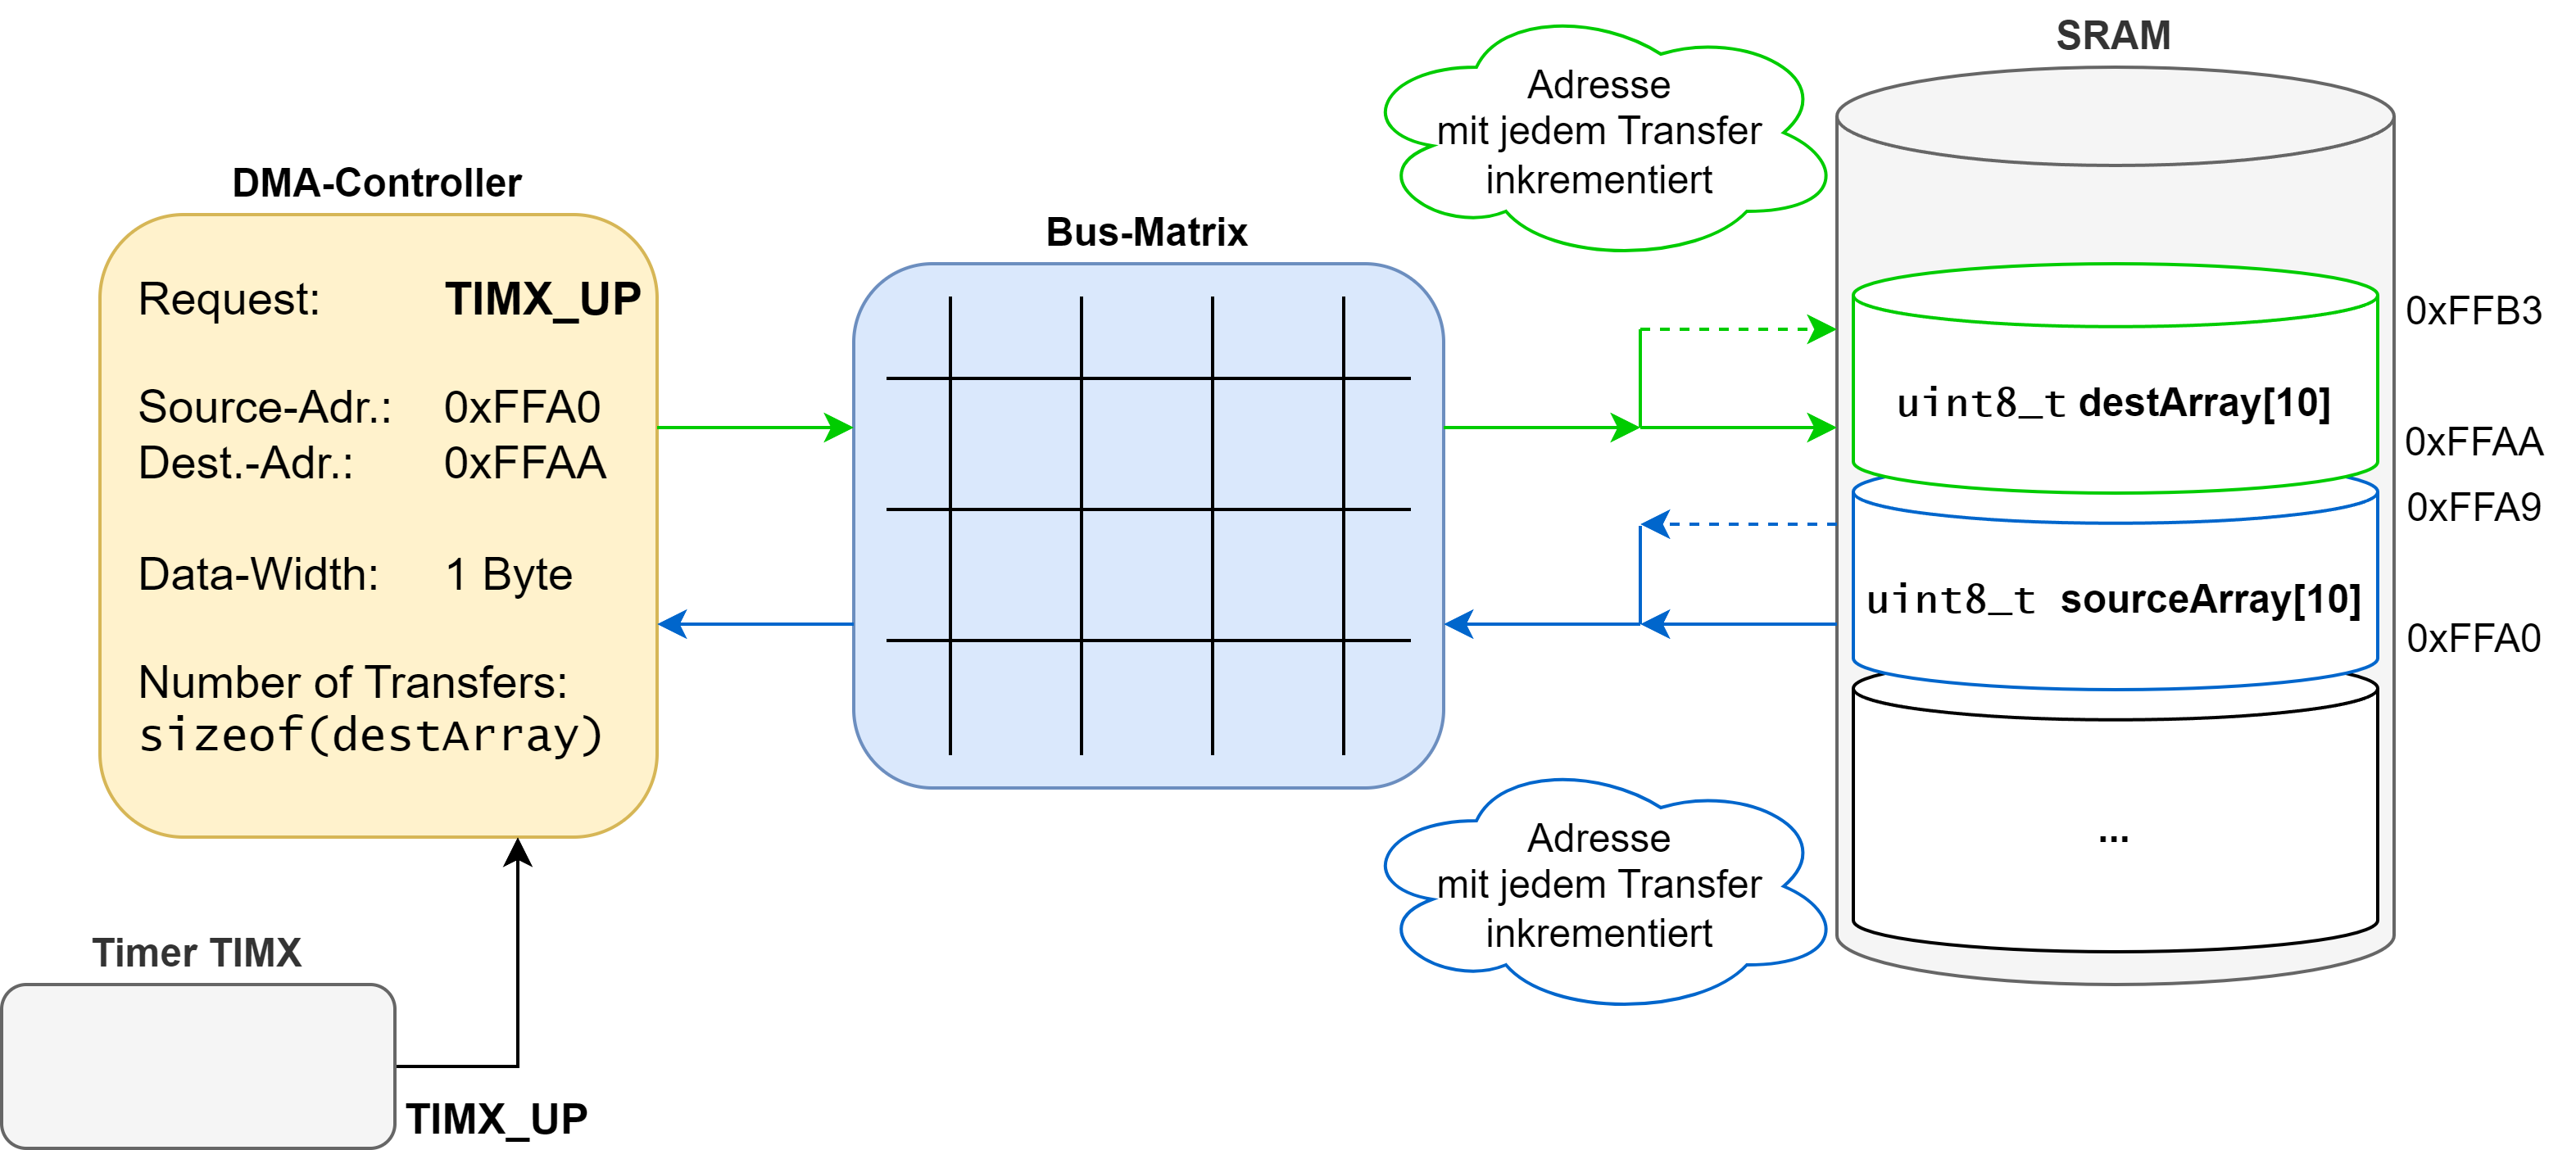
\includegraphics[scale=0.1]{Prinzip_periph2mem.png} 
	\caption{peripheral-to-memory-Transfer}
	\label{fig:periph_to_mem}
\end{figure}

Im Abtastsystem ist keine Inkrementierung der Quelladresse notwendig, da nur das Eingangsdatenregister ausgelesen werden muss, welches die Schnittstelle zum parallelen ADC-Interface darstellt (siehe \autoref{dma_data_acq} im Entwurfsteil der FW).

\pagebreak

\textbf{\underline{DMA-Transferwege}}\\

Gemeinsames Übertragungsmedium ist die Bus-Switch-Matrix, die auch in den vorherigen Abbildungen schon dargestellt wurde. Der Zugriff auf diese wird mit Hilfe einer Arbitrierung nach einem round-robin-Algorithmus geregelt. 
Durch den Arbitrierungsvorgang oder die Blockierung des Übertragungsmediums durch einen anderen Bus-Master (z.B. die CPU) kann eine \emph{Latenz beim DMA-Transfer} entstehen.

\begin{figure}[H]
	\centering
    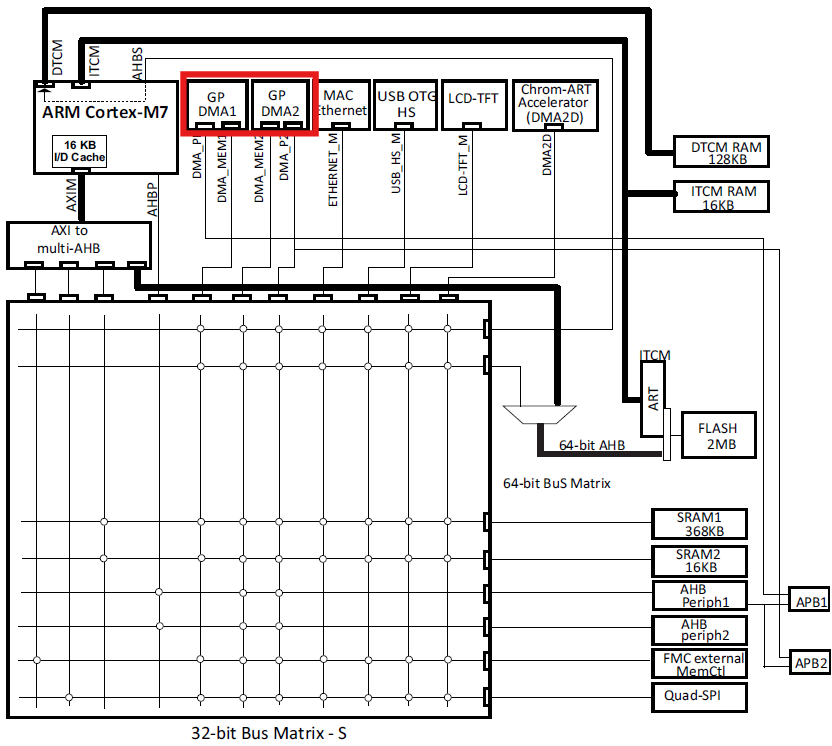
\includegraphics[scale=0.7]{Systemarchitektur_STM32F7.png} 
	\caption{Systemarchitektur für STM32F76xxx $\mu$C aus \cite[S. 72]{STmicroelectronics2024}}
	\label{fig:sysarch_stm32f7}
\end{figure}

Nur Bus-Master (z.B.: Prozessor, DMA-Controller (in \autoref{fig:sysarch_stm32f7} rot hervorgehoben) können Lese- und Schreiboperationen initiieren.

\pagebreak

\subsection{Digitale Filterung (Preprocessing)}
\label{subsec:digital_filtering}
\href{https://www.analog.com/en/resources/technical-books/scientist_engineers_guide.html}{The Scientist \& Engineers Guide to Digital Signal Processing, 1999}

\pagebreak

%%%%%%%%%%% Projektkonzeption %%%%%%%%%%%
\section{Projektkonzeption}
\subsection{Vorgehensweise}
Das übergeordnete Vorgehen folgte einem strukturierten Prozess, der sich gut durch das \textbf{V-Modell} visualisieren lässt. Diese Vorgehensweise eignete sich insbesondere aus drei Gründen: \emph{Erstens}, Änderungen an Hardware sind nach deren Umsetzung nur schwer möglich, was iterative Prozesse sehr aufwendig macht. \emph{Zweitens} standen die Projektziele von Beginn an eindeutig fest. \emph{Drittens} waren die Aufgabenbereiche klar voneinander abgegrenzt. Zudem handelte es sich um ein überschaubares Projekt.

\begin{figure}[H]
\centering
    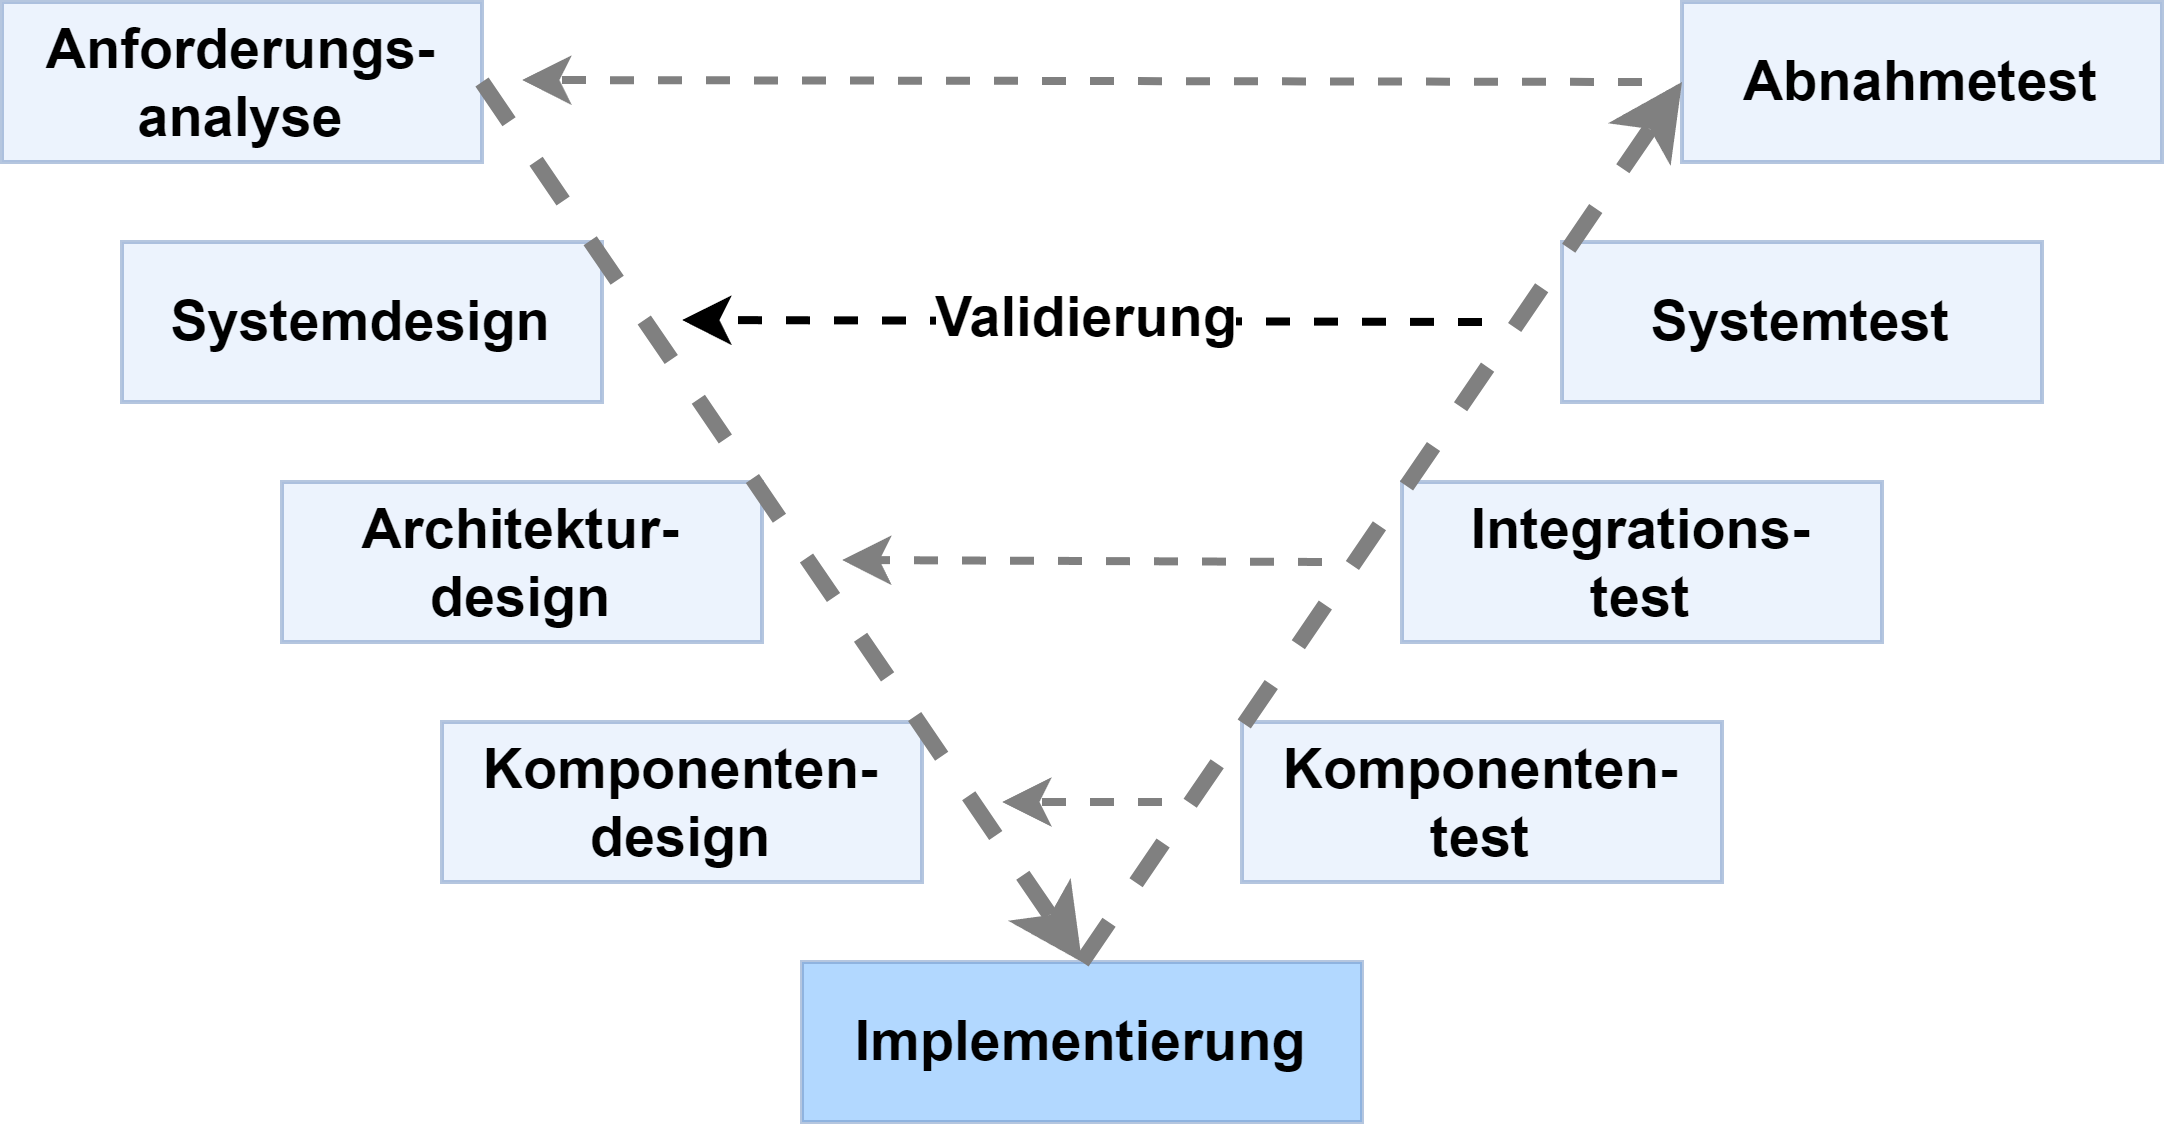
\includegraphics[scale=0.14]{V_Modell.png} 
	\caption{V-Modell}
\end{figure}

Im Folgenden werden die einzelnen Phasen und zugehörigen Validierungsschritte kurz erläutert.\vspace{0.1cm}\\
\underline{Anforderungsanalyse und Abnahmetest}\\
In enger Abstimmung mit dem betreuenden Professor wurden die grundlegenden Anforderungen definiert. Dazu gehörten unter anderem Bandbreite, Abtastrate, Auflösung und Eingangsspannungsbereich. Der spätere Abnahmetest bestand darin zu überprüfen, ob das entwickelte System diese Vorgaben in einer realistischen Versuchsumgebung erfüllte.\vspace{0.1cm}\\
\underline{Systemdesign und Systemtest}\\
Anschließend wurden die grundlegenden Systemfunktionen festgelegt, die zur Erfüllung der Anforderungen notwendig waren. Dazu zählten Signalaufnahme, Digitalisierung, Weiterleitung über USB und Visualisierung am PC. Im Systemtest wurde das fertige Gerät als Gesamtsystem geprüft.\vspace{0.1cm}\\
\underline{Architekturdesign und Integrationstest}\\
In dieser Phase erfolgte die Aufteilung des Systems in die Bereiche Hardware, Firmware und Software. Dabei wurden die Schnittstellen definiert, die ermöglichen sollten, die Module weitgehend unabhängig voneinander zu entwickeln. Diese wurden während des Komponentendesigns bei Bedarf konkretisiert. Im Integrationstest wurde die Zusammenarbeit dieser Module überprüft, insbesondere die zuverlässige Kommunikation zwischen den Subsystemen.\vspace{0.1cm}\\
\underline{Komponentendesign und Komponententest}\\
In dieser Phase wurden die Teilsysteme detailliert ausgearbeitet. Es wurden Konzepte erstellt, Bauteile gewählt, Implementierungsmöglichkeiten abgewogen etc. Jedes Subsystem wurde einzeln getestet, z. B. Spannungsversorgung und ADC in der Hardware, Speicherzugriffe in der Firmware oder Datenanzeige in der Software.\vspace{0.1cm}\\
\underline{Implementierung}\\
In der zentralen Phase wurden die geplanten Komponenten umgesetzt. Dies umfasste das Layout der Schaltungen, die Programmierung der Firmware sowie die Entwicklung der PC-Software. Ziel war es, die entworfenen Module funktionsfähig zu realisieren und für die Integration bereitzustellen.\\

\textbf{Organisation und Zusammenarbeit}\\
Die Zusammenarbeit erfolgte hauptsächlich über ein gemeinsames Projektteam in Microsoft Teams. Dieses war in mehrere Kanäle gegliedert: einen allgemeinen Kanal für projektübergreifende Informationen, jeweils eigene Kanäle für Hardware, Firmware und Software sowie zusätzliche Kanäle für die Schnittstellen. Diese Struktur erleichterte die Ablage von Quellen, Materialien und Informationen und stellte die Übersicht über das gesamte Projekt sicher.\\
Die Abstimmung innerhalb des Teams erfolgte in regelmäßigen Treffen, in denen abgeschlossene Arbeitspakete dokumentiert und neue Zielvorgaben bis zum nächsten Treffen festgelegt wurden. Die Ergebnisse wurden jeweils in Protokollen festgehalten. Eine detaillierte Auflistung der Tätigkeiten sowie deren Zuordnung zu den einzelnen Teammitgliedern findet sich im \nameref{sec:appendix_a} \ref{sec:appendix_a}.
\pagebreak

\subsection{Anforderungen}
Die Anforderungen an das Projekt wurden in Zusammenarbeit mit dem betreuenden Professor sowie dem Laboringenieur des MCT-Labors Hr. Lenkowski nach einer ersten Machbarkeitsanalyse im Hinblick auf die definierten Projektziele festgelegt. Neben den obligatorischen Grundfunktionen eines digitalen Speicheroszilloskops (siehe \autoref{subsec:oscilloscope_func} ``\nameref{subsec:oscilloscope_func}``) wurden folgende zentrale technische Parameter bestimmt:
\begin{itemize}
\item Bandbreite: 1 MHz (Grenzfrequenz des Anti-Aliasing-Filters)
\item Abtastrate: mindestens 10 MS/s (siehe \autoref{subsec:aaf_nyquist})
\item Auflösung: mindestens 10 Bit
\item Analoge Eingangsspannung: ± 5 V
\item Offset: ± 5 V (bezogen auf die Eingangsspannung)
\end{itemize}

Ein weiterer wesentlicher Aspekt war die \emph{Spannungsversorgung} des Systems, für die bewusst keine strikten Anforderungen formuliert wurden. Auf diese Weise sollte während des Entwicklungsprozesses ein höheres Maß an Flexibilität gewährleistet werden, um den Fokus auf die grundlegende Funktionalität des Gesamtsystems legen zu können. Die Signalaufnahme sollte auf \emph{einen Kanal} beschränkt bleiben, um Schwierigkeiten bei der Synchronisation mehrerer ADCs sowie den erhöhten Verwaltungsaufwand für Mehrkanalsysteme zu vermeiden. Außerdem sollte die Möglichkeit bestehen, dass Oszilloskop mit einem Standardtastkopf zu betreiben. Zusätzlich war vorgesehen, die Baugruppe als \emph{erweiterbares Steckboard für ein Mikrocontroller-Entwicklungsboard} umzusetzen, wodurch die Komplexität reduziert und die Funktionalität der Baugruppe in den Vordergrund gestellt werden konnte.\\

Für die Schnittstelle zwischen ADC und Mikrocontroller wurde eine \emph{parallele Anbindung} vorgesehen, da eine serielle Übertragung über SPI bei den geforderten Abtastraten eine zu hohe Taktfrequenz erfordert hätte. Dies hätte einen direkten Datentransfer in den Speicher des Mikrocontrollers nicht mehr zuverlässig ermöglicht. Für die zentrale Recheneinheit wurde sich auf die \emph{Mikrocontroller der STM32-Familie} beschränkt, um vorhandene Kenntnisse aus den Modulen Mikrocomputertechnik und Embedded Systems gezielt einsetzen zu können. Die Kommunikation mit dem PC sollte über eine \emph{USB-Schnittstelle} erfolgen, um eine möglichst uneingeschränkte Kompatibilität zu gewährleisten. Auf dem PC war die Entwicklung einer \emph{eigenen Anwendung zur Visualisierung und Verarbeitung der Messdaten} vorgesehen. Diese sollte über \emph{genormte Kommandos} kommunizieren, sodass auch eine Integration in gängige Entwicklungs- und Analyseumgebungen wie \emph{LabVIEW} oder \emph{MATLAB} möglich wäre.\\

Neben diesen zentralen Vorgaben wurden auch \emph{optionale Erweiterungen} definiert, die nicht als kritisch für den Projekterfolg eingestuft wurden oder den vorgesehenen Arbeitsumfang überschritten. Dazu zählten insbesondere die Implementierung eines \emph{Logikanalysators} mit Protokolldekodierung gängiger Schnittstellen (z. B. SPI, I²C, UART), die Realisierung einer \emph{Fast-Fourier-Transformation (FFT)} zur Spektrumanalyse, die Erweiterung um einen \emph{zweiten analogen Kanal}, die Integration von \emph{Mathematik- und Messfunktionen} sowie die Nutzung unterschiedlicher \emph{Triggerbedingungen}. Weitere Optionen im Hardwarebereich betrafen eine \emph{Optimierung hinsichtlich elektromagnetischer Verträglichkeit (EMV)}, eine \emph{Minimierung des Rauschverhaltens}, die \emph{Stromversorgung über USB} sowie die \emph{Integration des Mikrocontrollers direkt auf der Baugruppe}.

\subsection{Konzept / Architektur}
Parallel zu den Anforderungen wurde ein Konzept entwickelt, um die grundlegende Architektur und Aufgabenverteilung des Projekts festzulegen. Zu Beginn entstand ein grundlegendes, rein funktionales Übersichtsbild (siehe \autoref{fig:block_concept}). Dieses stellt die wesentlichen Signalflüsse und Verarbeitungsschritte dar, die für die Realisierung des USB-Oszilloskops erforderlich sind. Der Signalpfad führt dabei vom Device under Test (DUT) über die Signalerfassung zur Speicherung der Rohdaten und weiter zur Verarbeitung auf PC-Ebene. Dieses Schema diente als Orientierungshilfe für die weiteren konzeptionellen Schritte, ohne jedoch bereits konkrete Funktionseinheiten Bauteile oder Schnittstellen festzulegen.\\

Auf Basis dieser funktionalen Skizze sowie des in der Fachliteratur beschriebenen Grundaufbaus eines digitalen Speicheroszilloskops (siehe \autoref{subsec:oscilloscope_func}) wurde schließlich ein Gesamtkonzept entwickelt, das Funktionseinheiten definiert und den jeweiligen Bereichen Hardware, Firmware und Software zuordnet (siehe \autoref{fig:complete_concept}).

\begin{figure}[H]
	\centering
    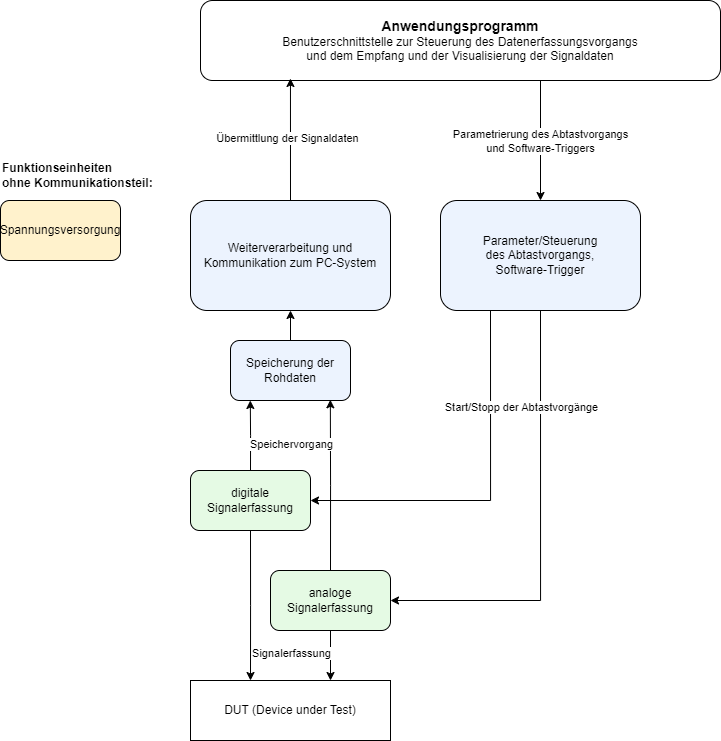
\includegraphics[scale=0.4]{Projektarbeit_Architektur.png} 
	\caption{Übersichts-Blockschaltbild (erstellt für die Konzeptvorstellung)}
	\label{fig:block_concept}
\end{figure}

\begin{figure}[H]
	\centering
    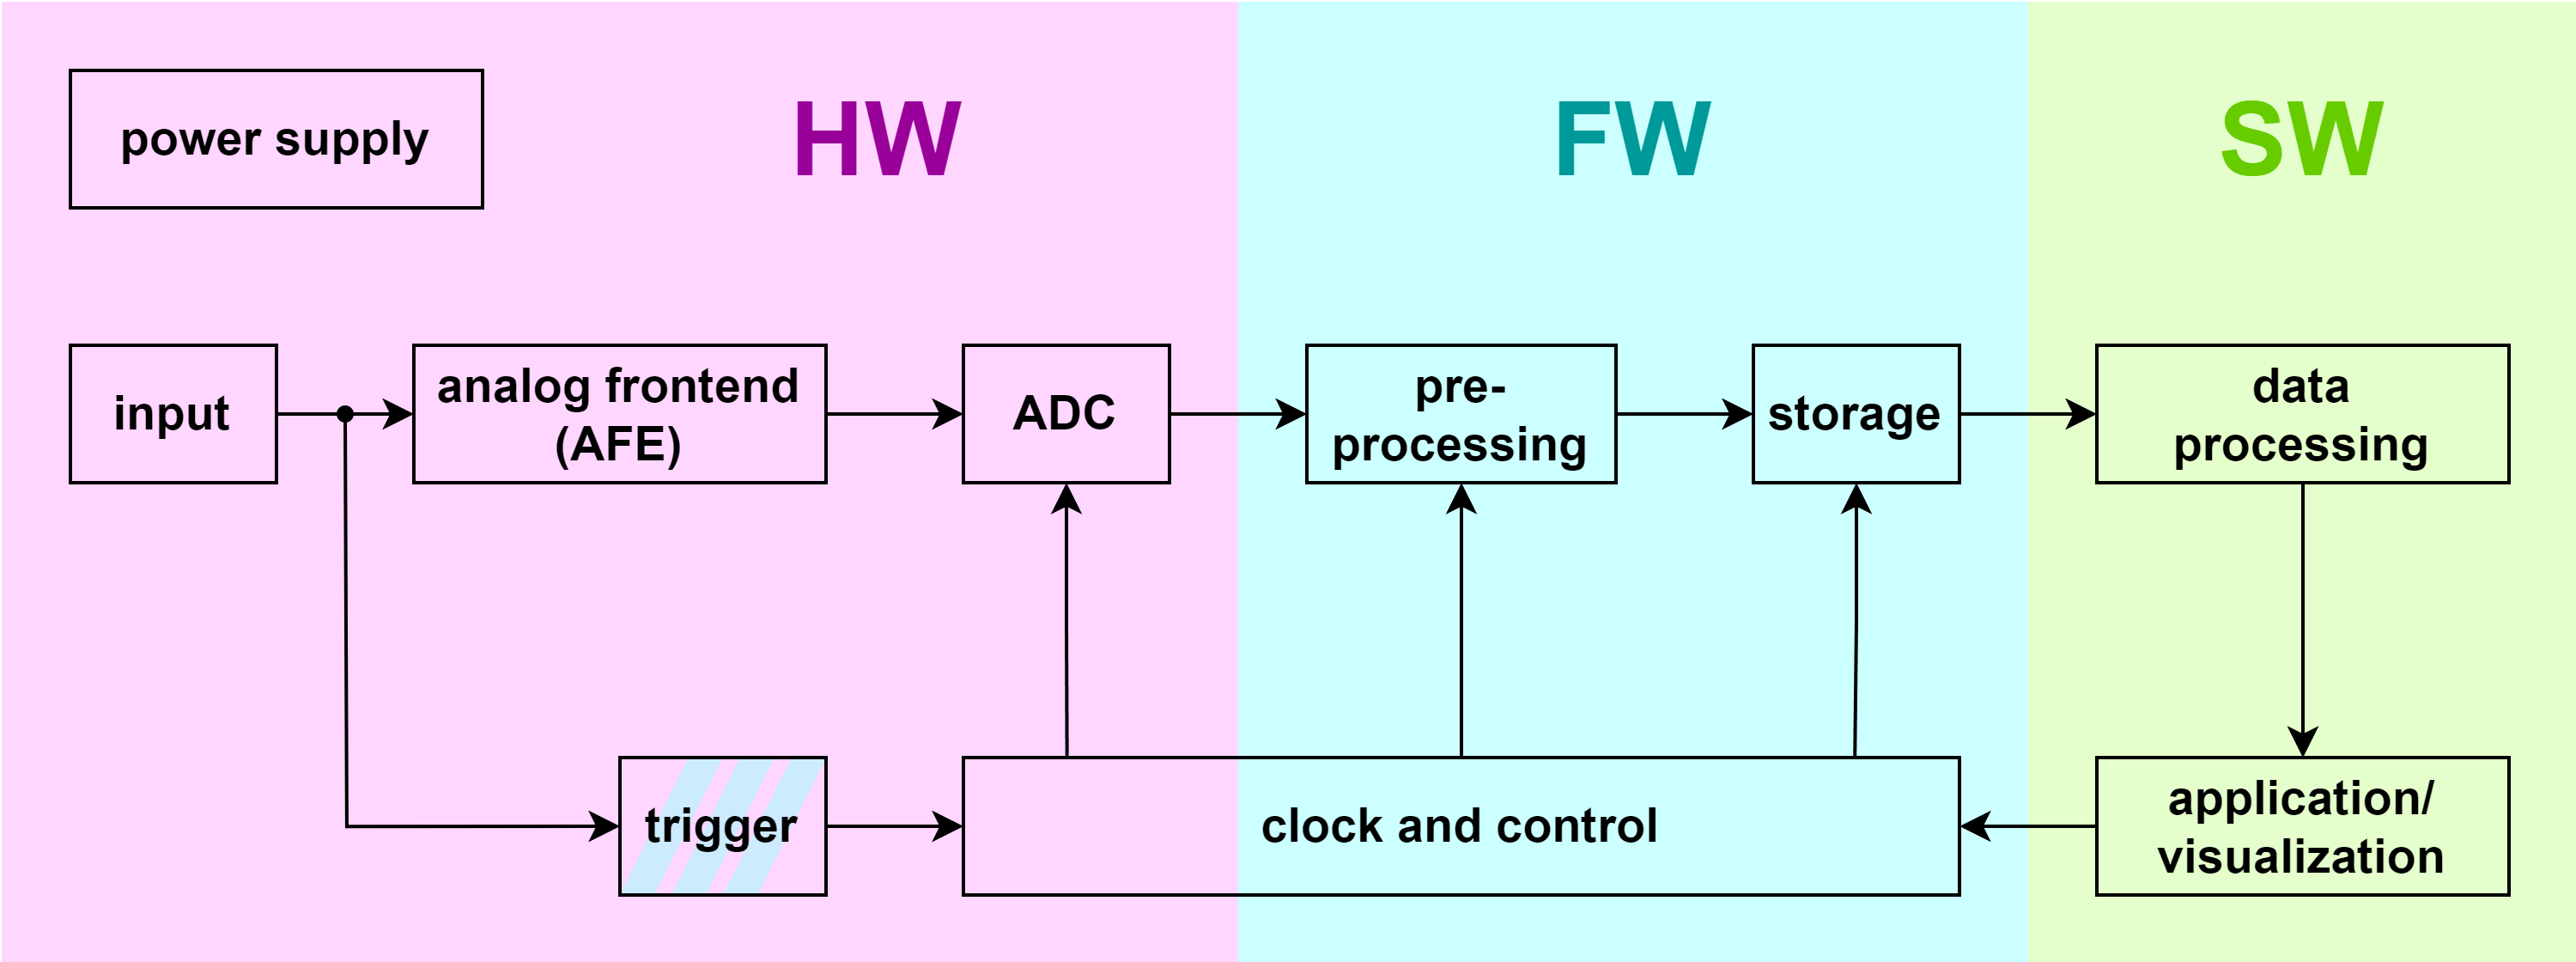
\includegraphics[scale=0.14]{Projektstruktur.png} 
	\caption{Gesamtkonzept des USB-Oszilloskops (nach \cite[S. 216]{Muehl2020})}
	\label{fig:complete_concept}
\end{figure}

Ausgehend von diesem Konzept und der klaren Aufteilung in die Bereiche Hardware, Firmware und Software, wurden die entsprechenden Schnittstellen festgelegt und die Aufgabenbereiche verteilt.

\pagebreak

%%%%%%%%%%% Realisierung %%%%%%%%%%%
\section{Hardware (HW)}
\subsection{Entwurf}
\subsection{Implementierung}
\subsection{HW-Test}

\pagebreak

\section{Schnittstelle Hardware - Firmware}

\pagebreak


\section{Firmware (FW)}
\subsection{Entwurf}
\subsubsection{Auswahl des Mikrocontrollers}
Eine zentrale Entscheidung im Entwurf der Firmware war die Auswahl eines geeigneten Mikrocontrollers (µC). Dieser stellt den zentralen Knotenpunkt der Gesamtanwendung dar. Hierzu wurden nach der Erstellung des Gesamtkonzepts zunächst die Anforderungen definiert, die an den Mikrocontroller gestellt werden.
Bei der Auswahl musste berücksichtigt werden, dass ein \emph{Direct Memory Access (DMA)} vorhanden ist. Dieser ermöglicht die Speicherung der Daten nach Eintreten eines Trigger-Ereignisses ohne Umweg über die CPU. Außerdem wurde gemäß der Anforderungen im Gesamtkonzept eine \emph{USB-Schnittstelle} benötigt, um die Kommunikation des Mikrocontrollers (USB-Device) mit dem PC (USB-Host) sicherzustellen. Dabei war es von Vorteil, wenn der Controller mindestens Full-Speed-Übertragungen mit 12 Mbit/s, idealerweise High-Speed-Übertragungen mit 480 Mbit/s unterstützt. Weiterhin war es erforderlich, dass ein \emph{erschwingliches Entwicklungsboard} verfügbar ist, welches für den ersten Prototypen genutzt werden kann. Dieses sollte zunächst zum Einsatz kommen, bevor der Mikrocontroller zusammen mit den übrigen Schaltungsteilen auf eine gemeinsame Leiterplatte integriert wird. Darüber hinaus sollten \emph{standardisierte Schnittstellen} wie I²C und SPI vorhanden sein, um die Anbindung eines externen ADCs auch auf andere Weise zu ermöglichen, falls die parallele Schnittstelle nicht umsetzbar wäre. Ein \emph{hoher GPIO Input Speed} war notwendig, um die geplante parallele Anbindung eines externen ADCs mit 12 Bit Auflösung über zwölf parallele GPIO-Leitungen bei der geplanten Abtastrate zu gewährleisten. Außerdem musste der Mikrocontroller über \emph{ausreichend großen SRAM-Speicher} verfügen, um die erfassten Abtastwerte ablegen zu können.

\begin{footnotesize}
	\begin{equation}
	[Benötigter Speicher] = [Anzahl Abtastwerte]\cdot \left[\frac{2 Byte}{Abtastwert}\right]
\end{equation}
\begin{equation}
	[Anzahl Abtastwerte] = \frac{[gewünschte Abtastzeit]}{[Abtastperiode]}
\end{equation}
\end{footnotesize}

Die Anforderungen wurde unter der Annahme formuliert, dass ein externer ADC eingesetzt werden sollte. Die angestrebte Abtastrate von etwa 10 MHz musste auch mikrocontrollerseitig erreichbar sein.\\

Auf Grundlage der positiven Erfahrungen mit STM32-Mikrocontrollern der Firma STMicroelectronics sowie der integrierten Entwicklungsumgebung STM32CubeIDE im MCT-Praktikum, wurde entschieden, einen Mikrocontroller aus dieser Serie auszuwählen. Ein zusätzlicher Vorteil dieser Produktfamilie ist die Verfügbarkeit kostengünstiger Entwicklungsboards (NUCLEO-Boards), die sich hervorragend für die ersten Entwicklungsschritte eignen und die Materialkosten des Projekts reduzieren.\\

Nach einem Vergleich verschiedener STM32-Produktfamilien in Bezug auf die definierten Anforderungen fiel die Wahl auf die \href{https://www.st.com/en/microcontrollers-microprocessors/stm32f7-series.html}{STM32F7-Serie}. Diese Mikrocontroller basieren auf einem ARM Cortex-M7 und gehören zum High-Performance-Bereich der STM32-Serie. Lediglich die STM32H7-Serie bietet noch höhere Leistung, da sie über einen weiteren Prozessorkern (Cortex-M4-Core) verfügen. Schlussendlich wurde der \href{https://www.st.com/en/microcontrollers-microprocessors/stm32f767zi.html}{STM32F767ZI} als Mikrocontroller ausgewählt. Dieser bietet im Vergleich zu anderen Controllern derselben Familie einen größeren Flash- und SRAM-Speicher. Zudem ist ein passendes Entwicklungsboard, das \href{https://www.st.com/en/evaluation-tools/nucleo-f767zi.html}{NUCLEO-F767ZI}, verfügbar. Ein weiterer Vorteil dieses Boards ist das integrierte Programmiergerät, das durch einen separaten Mikrocontroller mit entsprechender Firmware realisiert wird.\\

\begin{figure}[H]
	\centering
    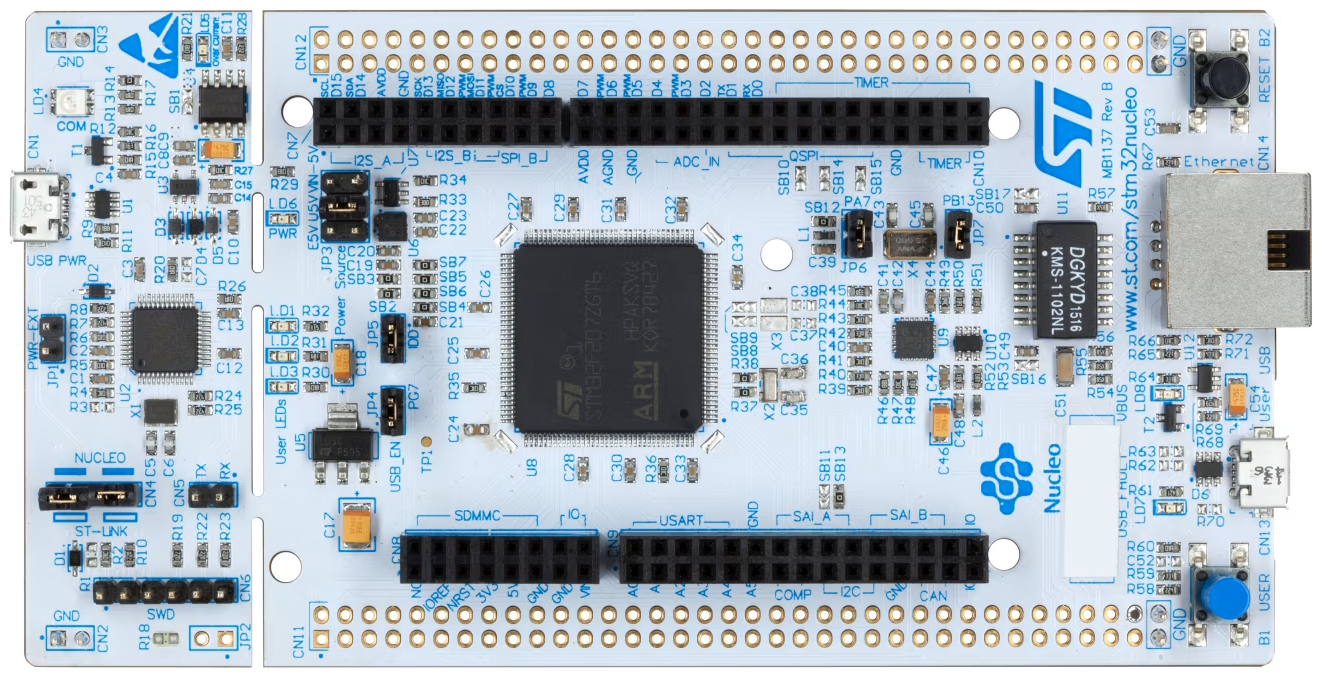
\includegraphics[scale=0.2]{nucleof767zi.png} 
	\caption{\centering Beispielabbildung für ein NUCLEO-144-Board, wie das NUCLEO-F767ZI\\ (Quelle: \href{https://www.st.com/en/evaluation-tools/nucleo-f767zi.html}{[Link]})}
	\label{fig:nucleo144}
\end{figure}

Nachdem die Entwicklungsboards in Absprache mit dem MCT-Labor beschafft worden waren, erfolgte eine erneute Einarbeitung in die Arbeit mit ARM Cortex-M Mikrocontrollern und den spezifischen Funktionen der STM32-Hardware.
\pagebreak

\subsubsection{Konzept des Abtastprozesses}
Der mikrocontrollerseitige Abtastprozess gliedert sich in zwei Hauptaufgaben:

\begin{itemize}
	\item Das \emph{Feststellen des Aufzeichnungsbeginns} durch ein definiertes Triggerereignis und

	\item die \emph{Aufnahme und Speicherung} der digitalisierten Abtastwerte.
\end{itemize}

Das Konzept der Abtastung ist als Funktionsschema in \autoref{fig:data_acq_concept} dargestellt.

\begin{figure}[H]
	\centering
    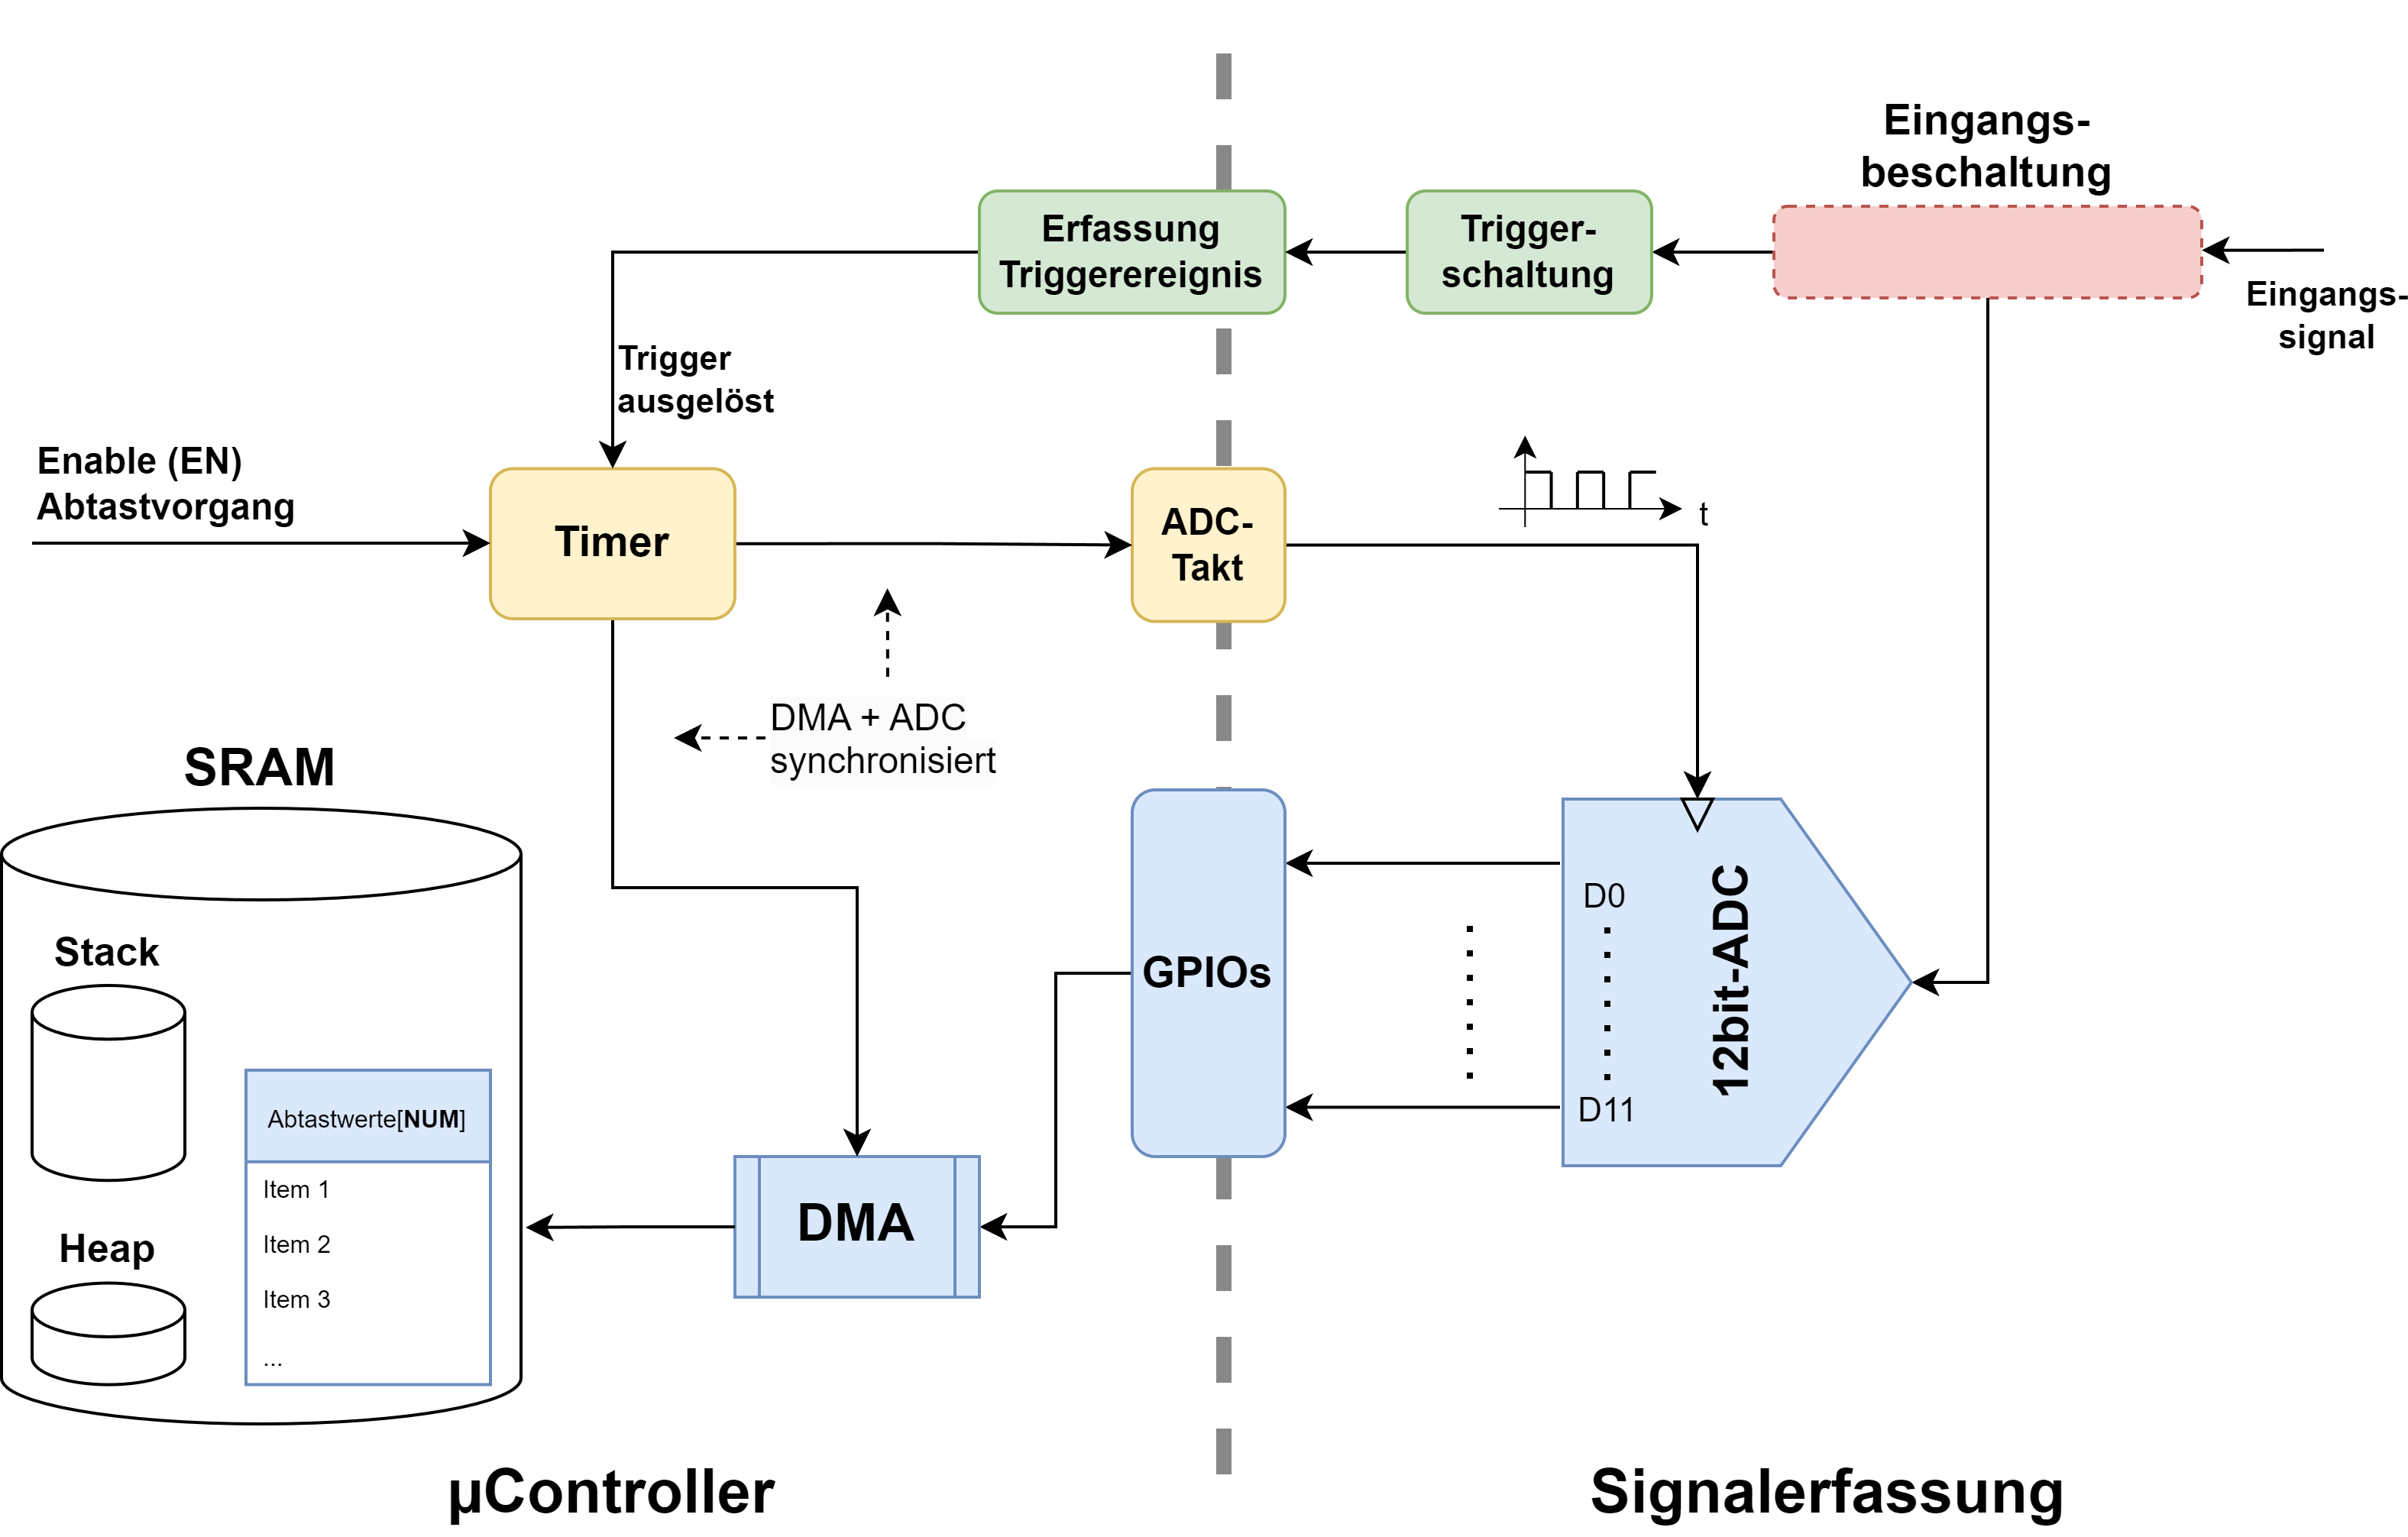
\includegraphics[scale=0.12]{Funktionsschema_Datenerfassung.png} 
	\caption{Funktionsschema der Abtastung}
	\label{fig:data_acq_concept}
\end{figure}

\underline{Parallele Datenanbindung}\\
Für die Übertragung der Messdaten vom externen ADC zum Mikrocontroller wurde eine \emph{parallele Schnittstelle} umgesetzt. Jedes der zwölf Bits des 12-Bit-ADCs wird dabei über eine eigene Datenleitung an den Mikrocontroller herangeführt. Der wesentliche Vorteil dieser Anbindung liegt in der vergleichsweise einfachen Implementierung, da kein komplexes serielles Übertragungsprotokoll notwendig ist. Ein Nachteil besteht jedoch darin, dass bei hohen Abtastraten Synchronisationsprobleme auftreten können.\\

Die GPIO-Pins des Mikrocontrollers sind in Ports mit jeweils 16 Pins organisiert, die sich ein gemeinsames \emph{Input Data Register (IDR)} teilen. Da für die Parallelschnittstelle zwölf Leitungen benötigt werden, können alle Bits der ADC-Ausgabe in einem einzigen Lesezugriff erfasst werden. Die Aktualisierung des IDR erfolgt mit jedem Zyklus des AHB-Busses \cite[S. 224]{STmicroelectronics2024}, der mit bis zu 216 MHz betrieben werden kann (siehe Clock-Tree in \cite[S. 154]{STmicroelectronics2024}). Dieser Wert wird aber durch eine vorhandene Eingangskapazität der GPIOs reduziert, welche eventuell auf einen neuen Wert (Spannungspegel) umgeladen werden müssen. Die tatsächliche, maximal mögliche Abtastfrequenz hängt also von dieser Eingangskapazität und der treibenden Schaltung ab. Im Datenblatt des $\mu$C ist für die Eingangskapazität ein Wert von $C_{IO}=5pF$ angegeben (\cite[S. 157]{STmicroelectronics2025}). Maximale Änderungsfrequenzen sind aber nur für die Nutzung der GPIOs als Output angegeben (die treibende Stufe ist dann die Ausgangsstufe des GPIO). Hier werden, je nach Einstellung des GPIO-Speeds (konfigurierbar), selbst im langsamsten Modus noch Frequenzen im einstelligen MHz-Bereich erreicht (\cite[S. 160f]{STmicroelectronics2025}). Unter der Annahme, dass die Treiberfähigkeit der ADC-Datenausgänge höher ist, kann die Abtastrate von 10 MHz realisiert werden.\\

\underline{Speicherorganisation}\\
Die erfassten Abtastwerte werden zunächst im internen SRAM des Mikrocontrollers zwischengespeichert. Der STM32F767 verfügt über insgesamt 512 KB SRAM, aufgeteilt in mehrere Speicherblöcke \cite[S. 77ff]{STmicroelectronics2024} (Memory Map). Für das Projekt wurde zunächst der \emph{SRAM1-Bereich} (368 KB) für die Speicherung der Messdaten reserviert, während der \emph{DTCM-Bereich} (128 KB) für Stack und Heap vorgesehen wurde. Diese Aufteilung gewährleistet eine klare Trennung zwischen Programmdaten und Messwertspeicher und kann bei der Implementierung im Linker-Script festgelegt werden.\\

\underline{DMA-basierter Datentransfer}\\
Ein direkter Zugriff der CPU auf die GPIO-Datenregister und das anschließende Abspeichern der Daten in den SRAM würde den Prozessor vollständig auslasten und keine parallele Ausführung anderer Aufgaben ermöglichen. Aus diesem Grund wurde der Datentransfer mithilfe des Direct Memory Access (DMA) realisiert (siehe \autoref{subsec:dma}).\\

Beim gewählten Ansatz wurde der DMA-Controller so konfiguriert, dass er den Wert des Eingangsdatenregisters der GPIOs automatisch in den SRAM schreibt, ohne dass die CPU beteiligt ist (siehe Schema in \autoref{fig:data_acq_dma}). Jeder DMA-Transfer wird durch einen Hardware-Timer (TIM1) angestoßen. Dadurch kann eine exakte Synchronisation zwischen dem Clock-Signal des ADC und der Datenübertragung erreicht werden. Die Quelladresse bleibt während der gesamten Aufzeichnung konstant (Adresse des IDR), während die Zieladresse nach jedem Transfer um zwei Byte inkrementiert wird, um den nächsten Speicherplatz im SRAM anzusprechen.

\begin{figure}[H]
	\centering
    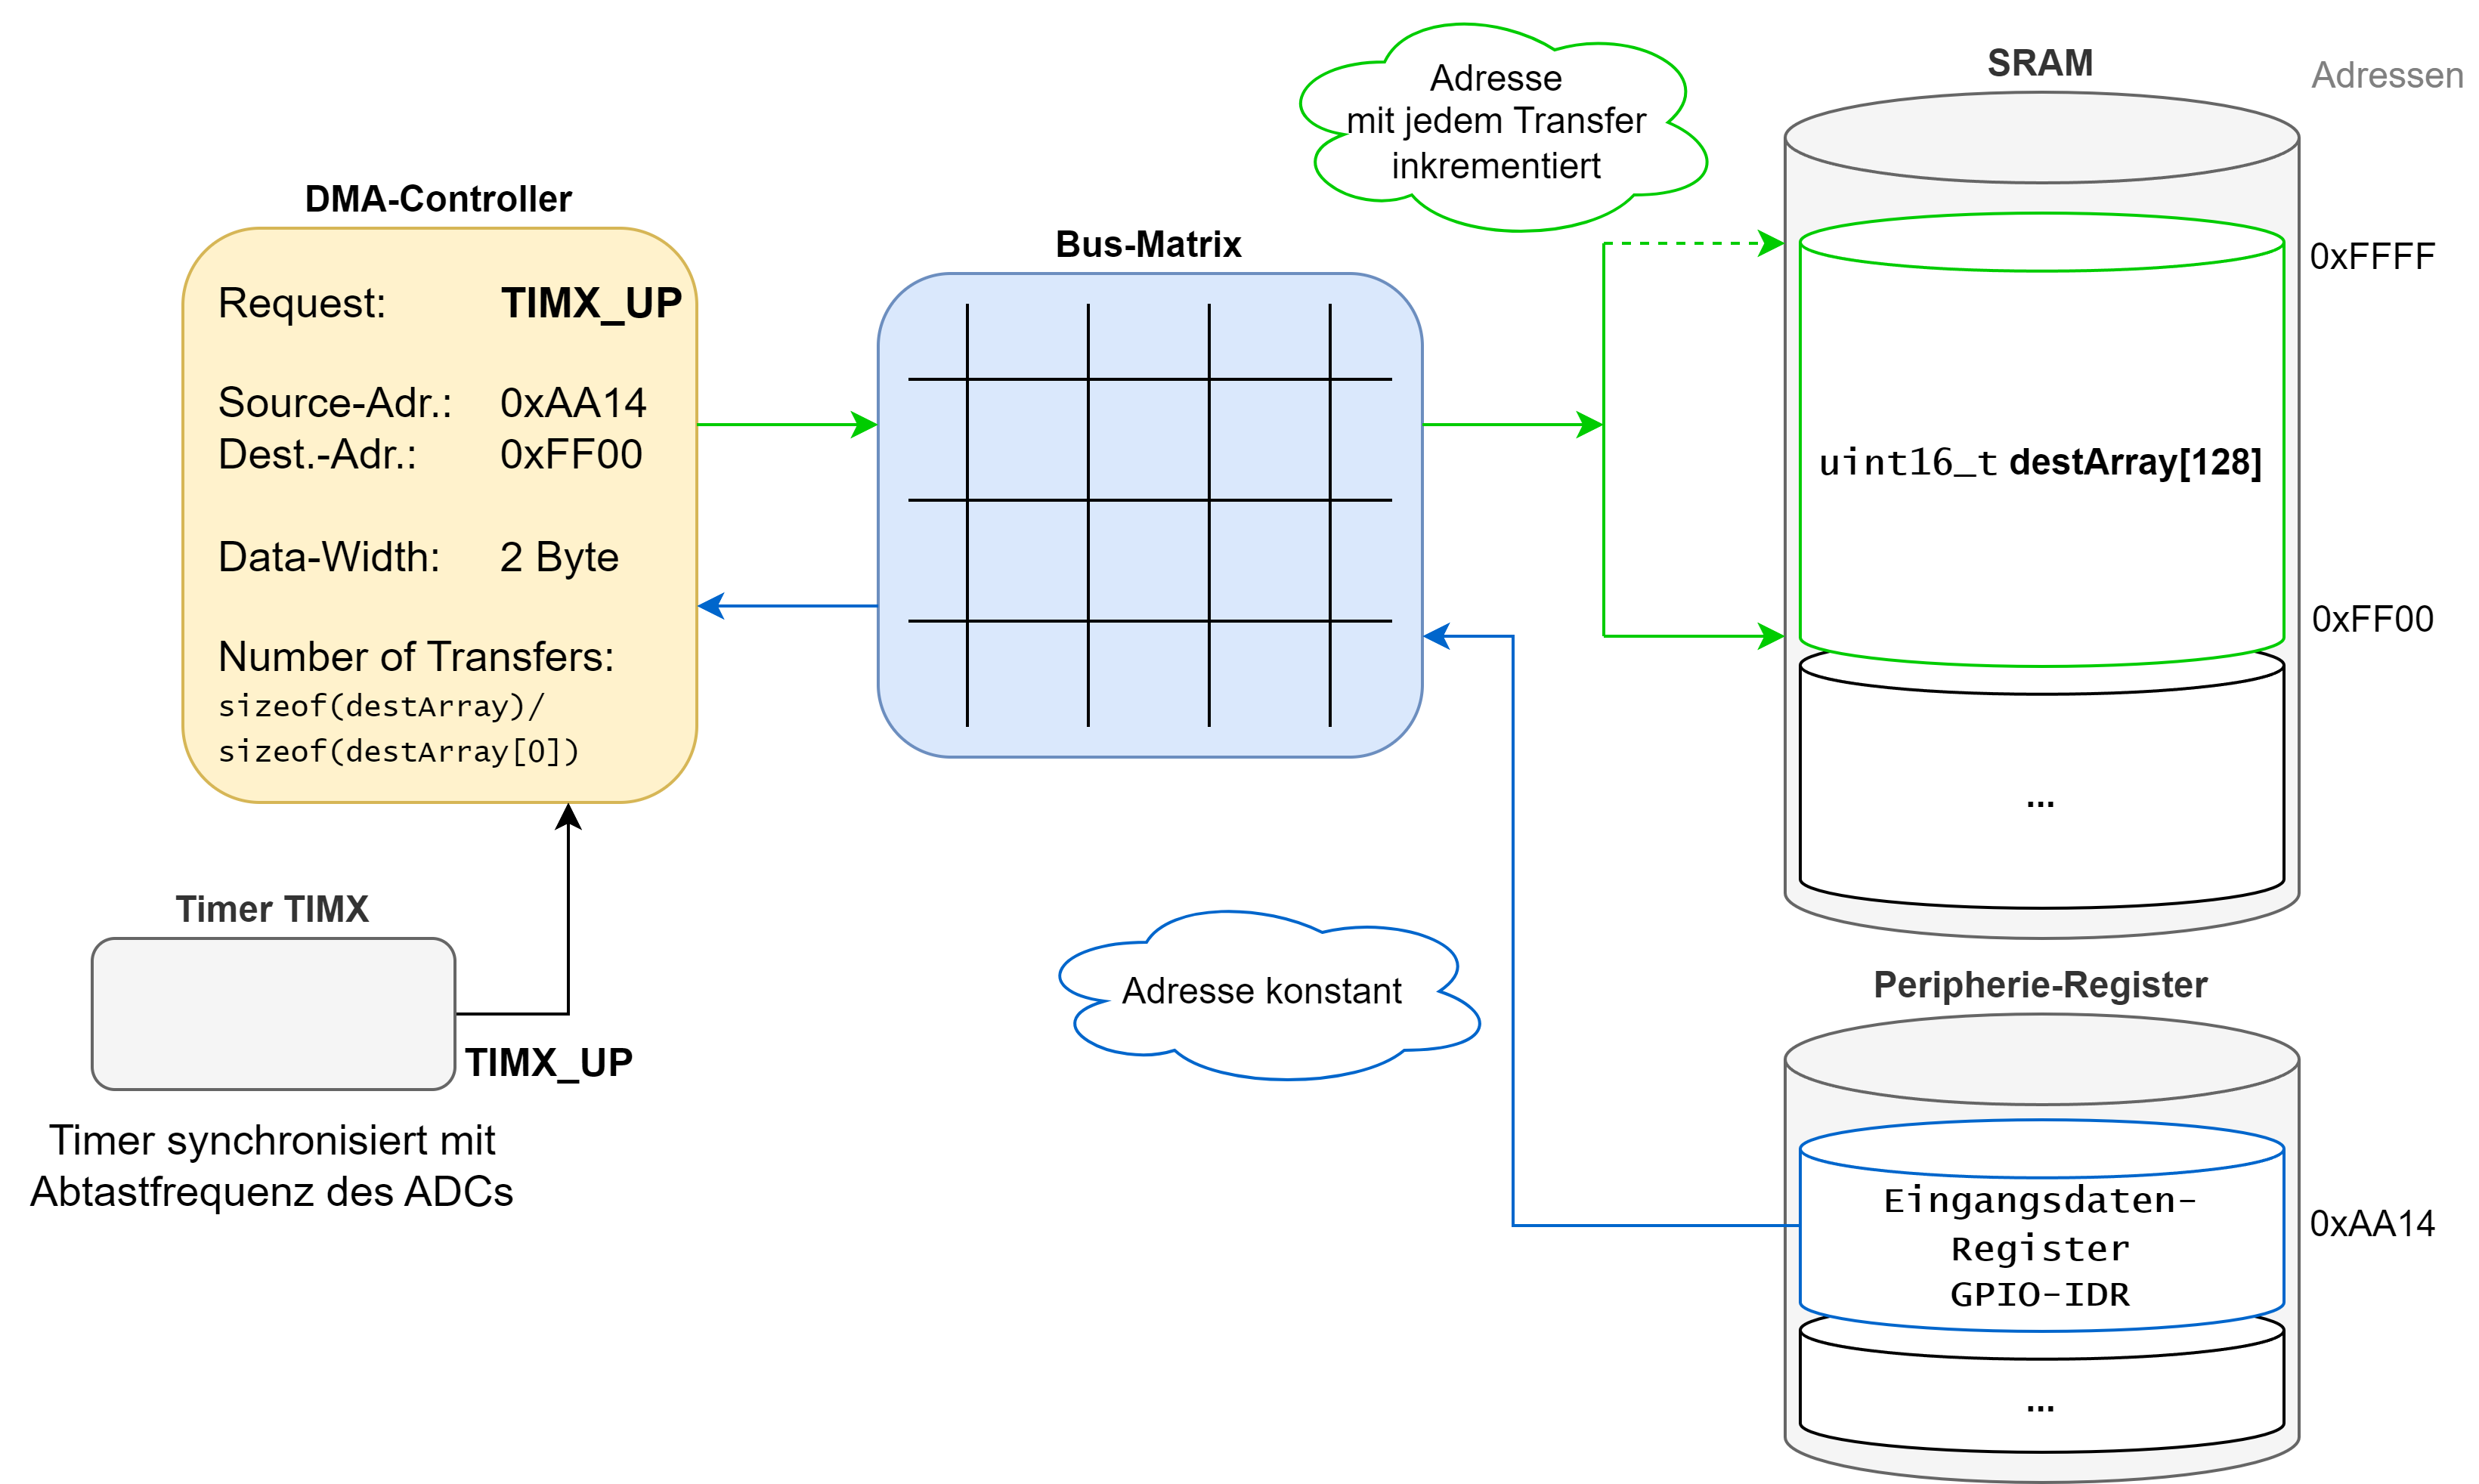
\includegraphics[scale=0.1]{Prinzip_DMA_Datenerfassung.png} 
	\caption{Funktionsprinzip DMA Abtastung - Adresswerte dienen nur der Übersicht}
	\label{fig:data_acq_dma}
\end{figure}

Da das NDTR-Register (Number of Data Transfers Register) maximal 65.535 Transfers speichern kann \cite[S. 276]{STmicroelectronics2024}, wird der Double-Buffer Mode (DBM) des DMA-Controllers eingesetzt (benötigt werden z.B. 100.000 Transfers für 100.000 Abtastwerte). In diesem Modus werden abwechselnd zwei getrennte Zieladress-Zeiger genutzt, um kontinuierliche Transfers ohne Datenverlust zu ermöglichen. Sobald ein Speicherbereich befüllt ist, wird automatisch in den anderen Bereich weitergeschrieben. Gleichzeitig kann die Software den gefüllten Speicherbereich auswerten oder für den USB-Transfer vorbereiten, ohne den laufenden Datentransfer zu unterbrechen.\\

\underline{Trigger-Mechnismus}\\
Der Beginn der Aufzeichnung wird durch ein definiertes Triggerereignis gesteuert. Nach dem Auslösen dieses Ereignisses startet der DMA automatisch mit dem Füllen des vorgesehenen Speicherbereichs. Die Größe dieses Bereichs sowie die Anzahl der Transfers wurde zuvor in der Firmware festgelegt. Sobald der Speicher vollständig gefüllt ist, wird der Abtastprozess automatisch beendet, und die Daten stehen für die anschließende Übertragung an den PC bereit. Der Trigger-Mechanismus wurde zunächst mit Hardware-Interrupts geplant (bei STM32: Extended Interrupts - EXTI). Mit dem EXTI-Modul kann ein Aufruf eines Exception-Handlers\footnote{Bezeichnung für eine Interrupt-Service-Routine (ISR) bei ARM-Cortex-$\mu$C.} bei einer steigenden oder fallenden Flanke an einem GPIO erfolgen, in welchem der DMA für die Datentransfers aktiviert wird\footnote{Die Zeit zwischen der Triggerflanke und DMA-Aktivierung im Exception-Handler ist die Triggerlatenz.}.\\

\underline{Synchronisation mit ADC-Takt}\\
Für eine störungsfreie Datenaufnahme muss der Datentransfer exakt auf den ADC-Takt abgestimmt werden. Hierfür wurde das Taktsignal für den ADC durch denselben Timer erzeugt, der auch die DMA-Requests auslöste. Die Hardware-Timer der STM32-Controller besitzen sogenannte Capture-Compare-Einheiten mit sogenannten Output-Compare-Anschlüssen (OC), welche mit bestimmten GPIOs des $\mu$C verbunden werden können (siehe \cite[S. 877]{STmicroelectronics2024}). Der Hardware-Timer kann hierdurch einen GPIO ohne CPU-Beteiligung ansteuern. Um ein Setup-Violation-Problem zu vermeiden, wurde der Takt invertiert: Die positive Flanke des Signals erzeugt am ADC-Ausgang einen neue Wert, während synchron zur negativen Flanke der DMA-Transfer ausgelöst wird. Dadurch können sich die ADC-Daten für eine halbe Abtastperiode $\frac{T_S}{2}$ stabilisieren, bevor sie eingelesen werden. Dies stellt eine zuverlässige Digitalisierung sicher (siehe \autoref{fig:timing_dma_adc}).

\begin{figure}[H]
	\centering
    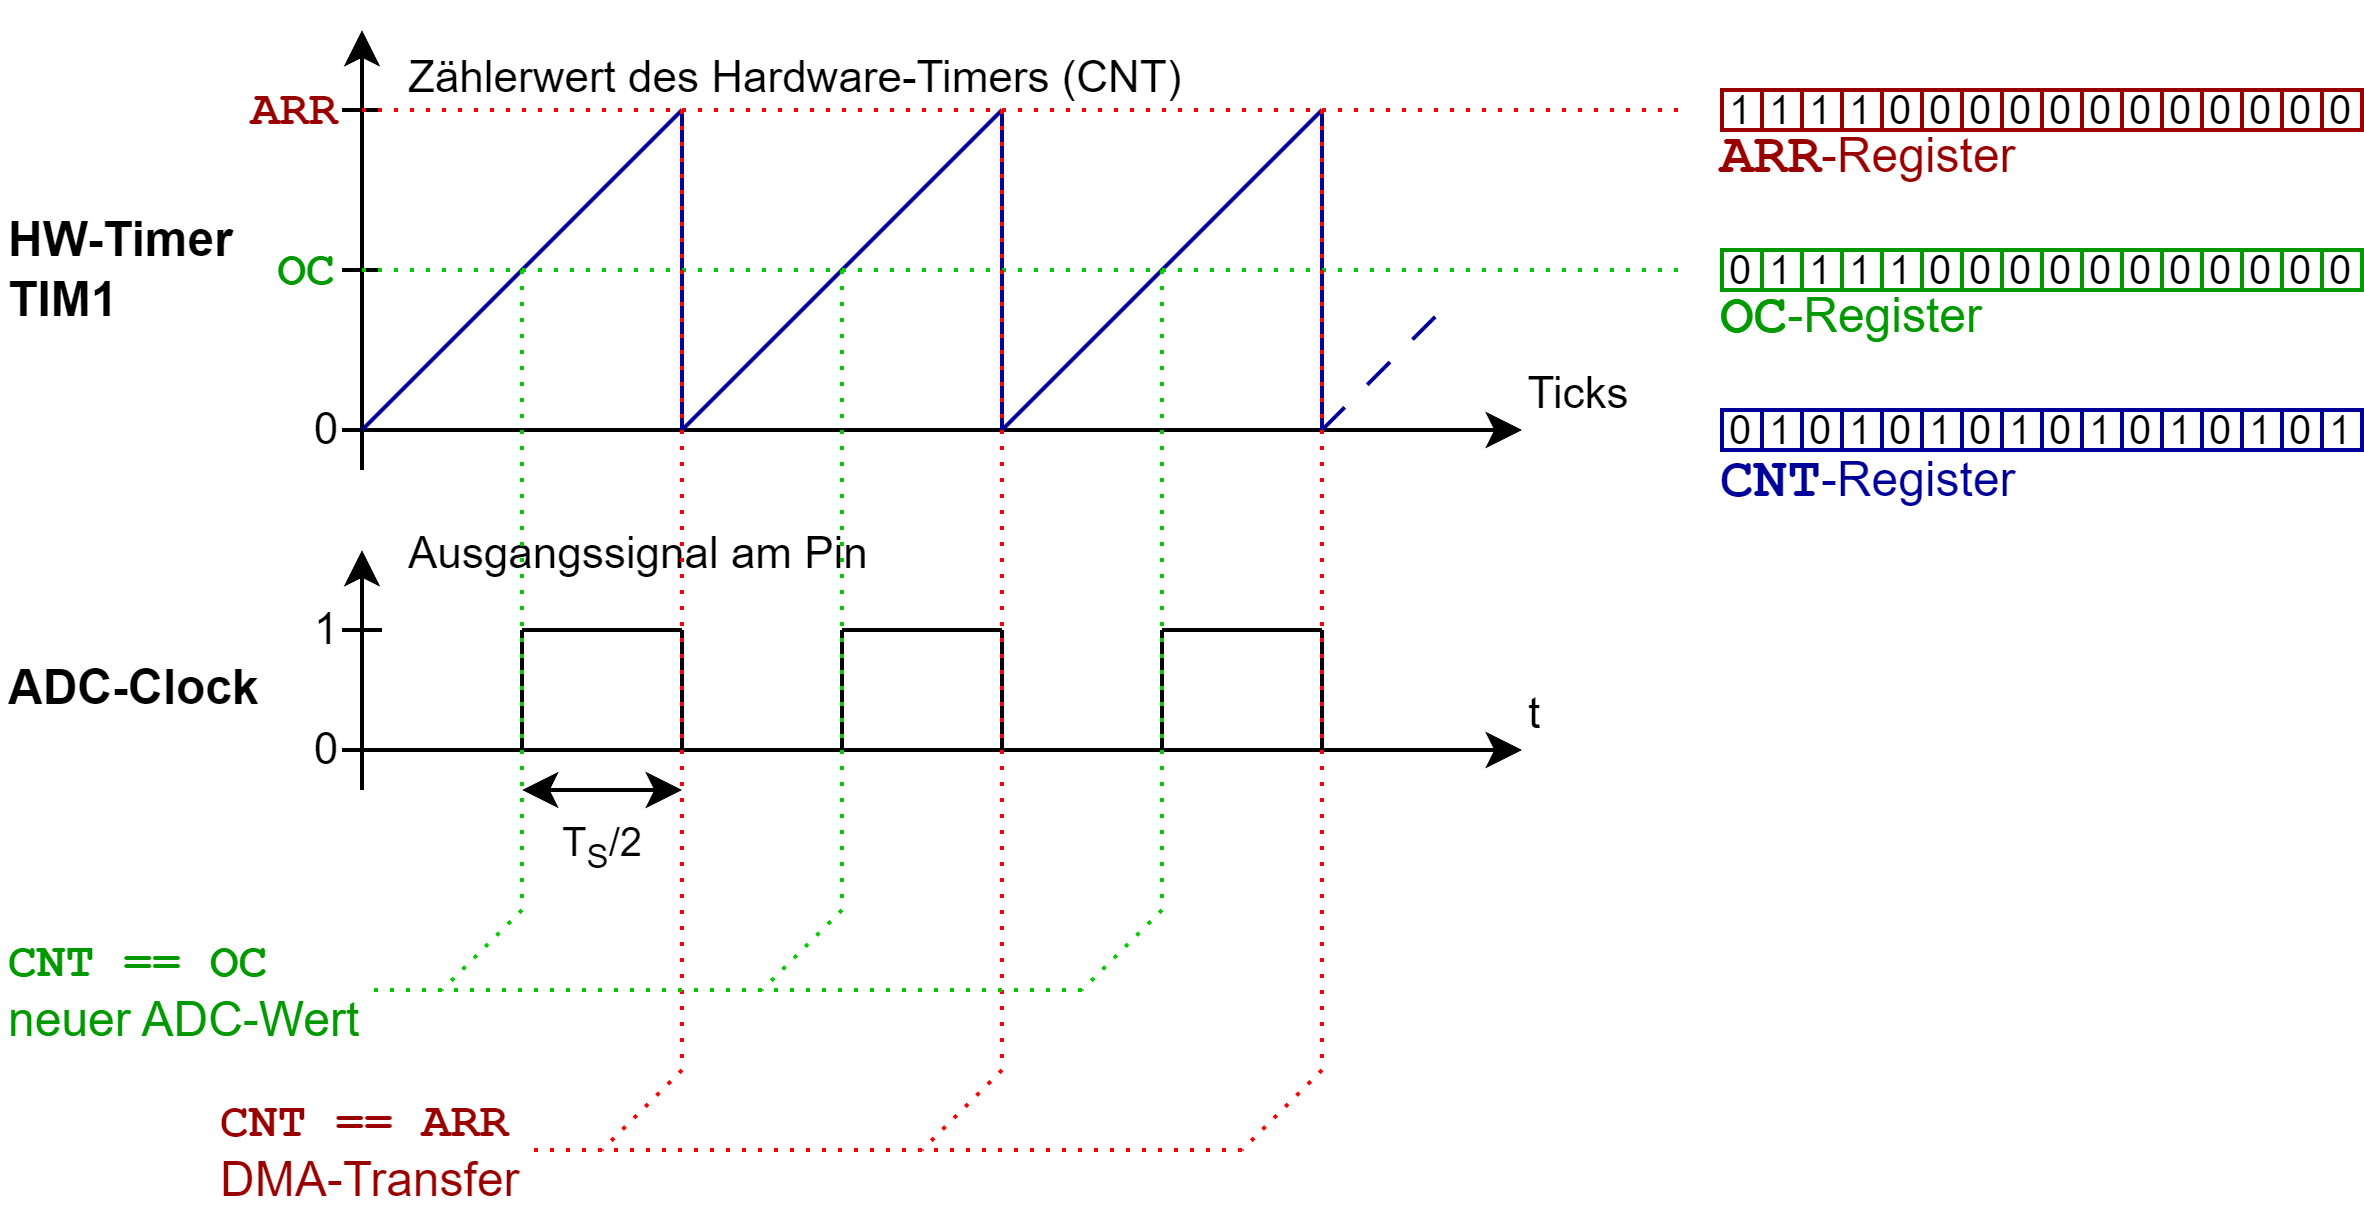
\includegraphics[scale=0.15]{Timing_Diagramm_Timer_ADC_DMA.png} 
	\caption{\centering Zeitdiagramm und Registerübersicht des Hardware-Timers\\für die Synchronisation von ADC und DMA (Sampling am $\mu$C)}
	\label{fig:timing_dma_adc}
\end{figure}

\pagebreak

\subsubsection{Konzept der Firmware als FSM}

\underline{Überblick}\\
Die Firmware des USB-Oszilloskops wurde auf der Basis einer Finite State Machine (FSM) zur Steuerung der Betriebszustände erstellt. Dieser Ansatz ermöglicht eine klare Trennung der verschiedenen Funktionsphasen sowie eine strukturierte und erweiterbare Implementierung. Die FSM verarbeitet asynchrone Ereignisse (Events; Präfix \texttt{EV\_}), die aus unterschiedlichen Quellen stammen können, wie z.B.:

\begin{itemize}
	\item Benutzereingaben (z. B. Button auf dem Board),
	\item Befehle der PC-Anwendung über USB,
	\item interne Signale der Hardware, wie z. B. Abschluss eines DMA-Transfers.
\end{itemize}

Die fachlichen Grundlagen zu FSMs wurden bereits in \autoref{subsec:fsm} erläutert.\\

Um diese Ereignisse effizient zu verarbeiten, wird eine Event-Queue verwendet. Jedes Event wird in diese Warteschlange (Queue) eingereiht („enqueued“). Die FSM verarbeitet die Ereignisse dann sequenziell, wodurch sichergestellt wird, dass auf asynchrone Signale deterministisch reagiert wird.\\

\underline{Architektur der FSM}\\
Die FSM besteht aus mehreren definierten Zuständen, die jeweils einer bestimmten Betriebsphase des Oszilloskops entsprechen. Jeder Zustand wird durch eine eigene Funktion realisiert. Diese Funktionen beinhalten drei Hauptbereiche:

\begin{enumerate}
	\item \emph{Entry-Block:}\\
	Wird beim Eintritt in einen Zustand ausgeführt (z. B. Initialisierungen, Statusmeldungen).

	\item \emph{Event-Handling:}\\
	Reaktion auf ankommende Events innerhalb des aktuellen Zustands.

	\item \emph{Exit-Block:}\\
	Wird beim Verlassen des Zustands ausgeführt (z. B. Aufräumarbeiten).
\end{enumerate}

Das State Diagram (siehe \autoref{fig:firmware_fsm}) visualisiert die Abfolge der Firmwarezustände sowie die möglichen Übergänge basierend auf bestimmten Events. Die Hauptzustände sind \autoref{table:states_firmware} zu entnehmen.
\pagebreak

\begin{table}[H]
\centering
\scriptsize
\begin{tabular}{|c|c|}
\hline 
\textbf{Zustand} & \textbf{Beschreibung} \\ 
\hline 
\hline
Init & Initialisierung der Hardware-Peripherie. Wird nur einmal beim Start ausgeführt. \\ 
\hline 
Idle & Warten auf Konfigurationsbefehle oder Startsignal der PC-Anwendung. \\ 
\hline 
Acquisition Start & Aktivieren des Triggers und Starten der Datenerfassung. \\ 
\hline 
Acquisition Done & Abschluss der Datenerfassung, Vorbereitung der Daten für die Übertragung. \\ 
\hline 
Data Transmission & Übertragung der erfassten Daten an den PC. \\ 
\hline 
Wait for ACK & Warten auf Bestätigung vom PC, ob ein weiterer Erfassungsvorgang gestartet werden soll. \\ 
\hline 
\end{tabular}
\caption{Übersicht über die Hauptzustände der Firmware-FSM}
\label{table:states_firmware}
\end{table}

\begin{figure}[H]
	\centering
    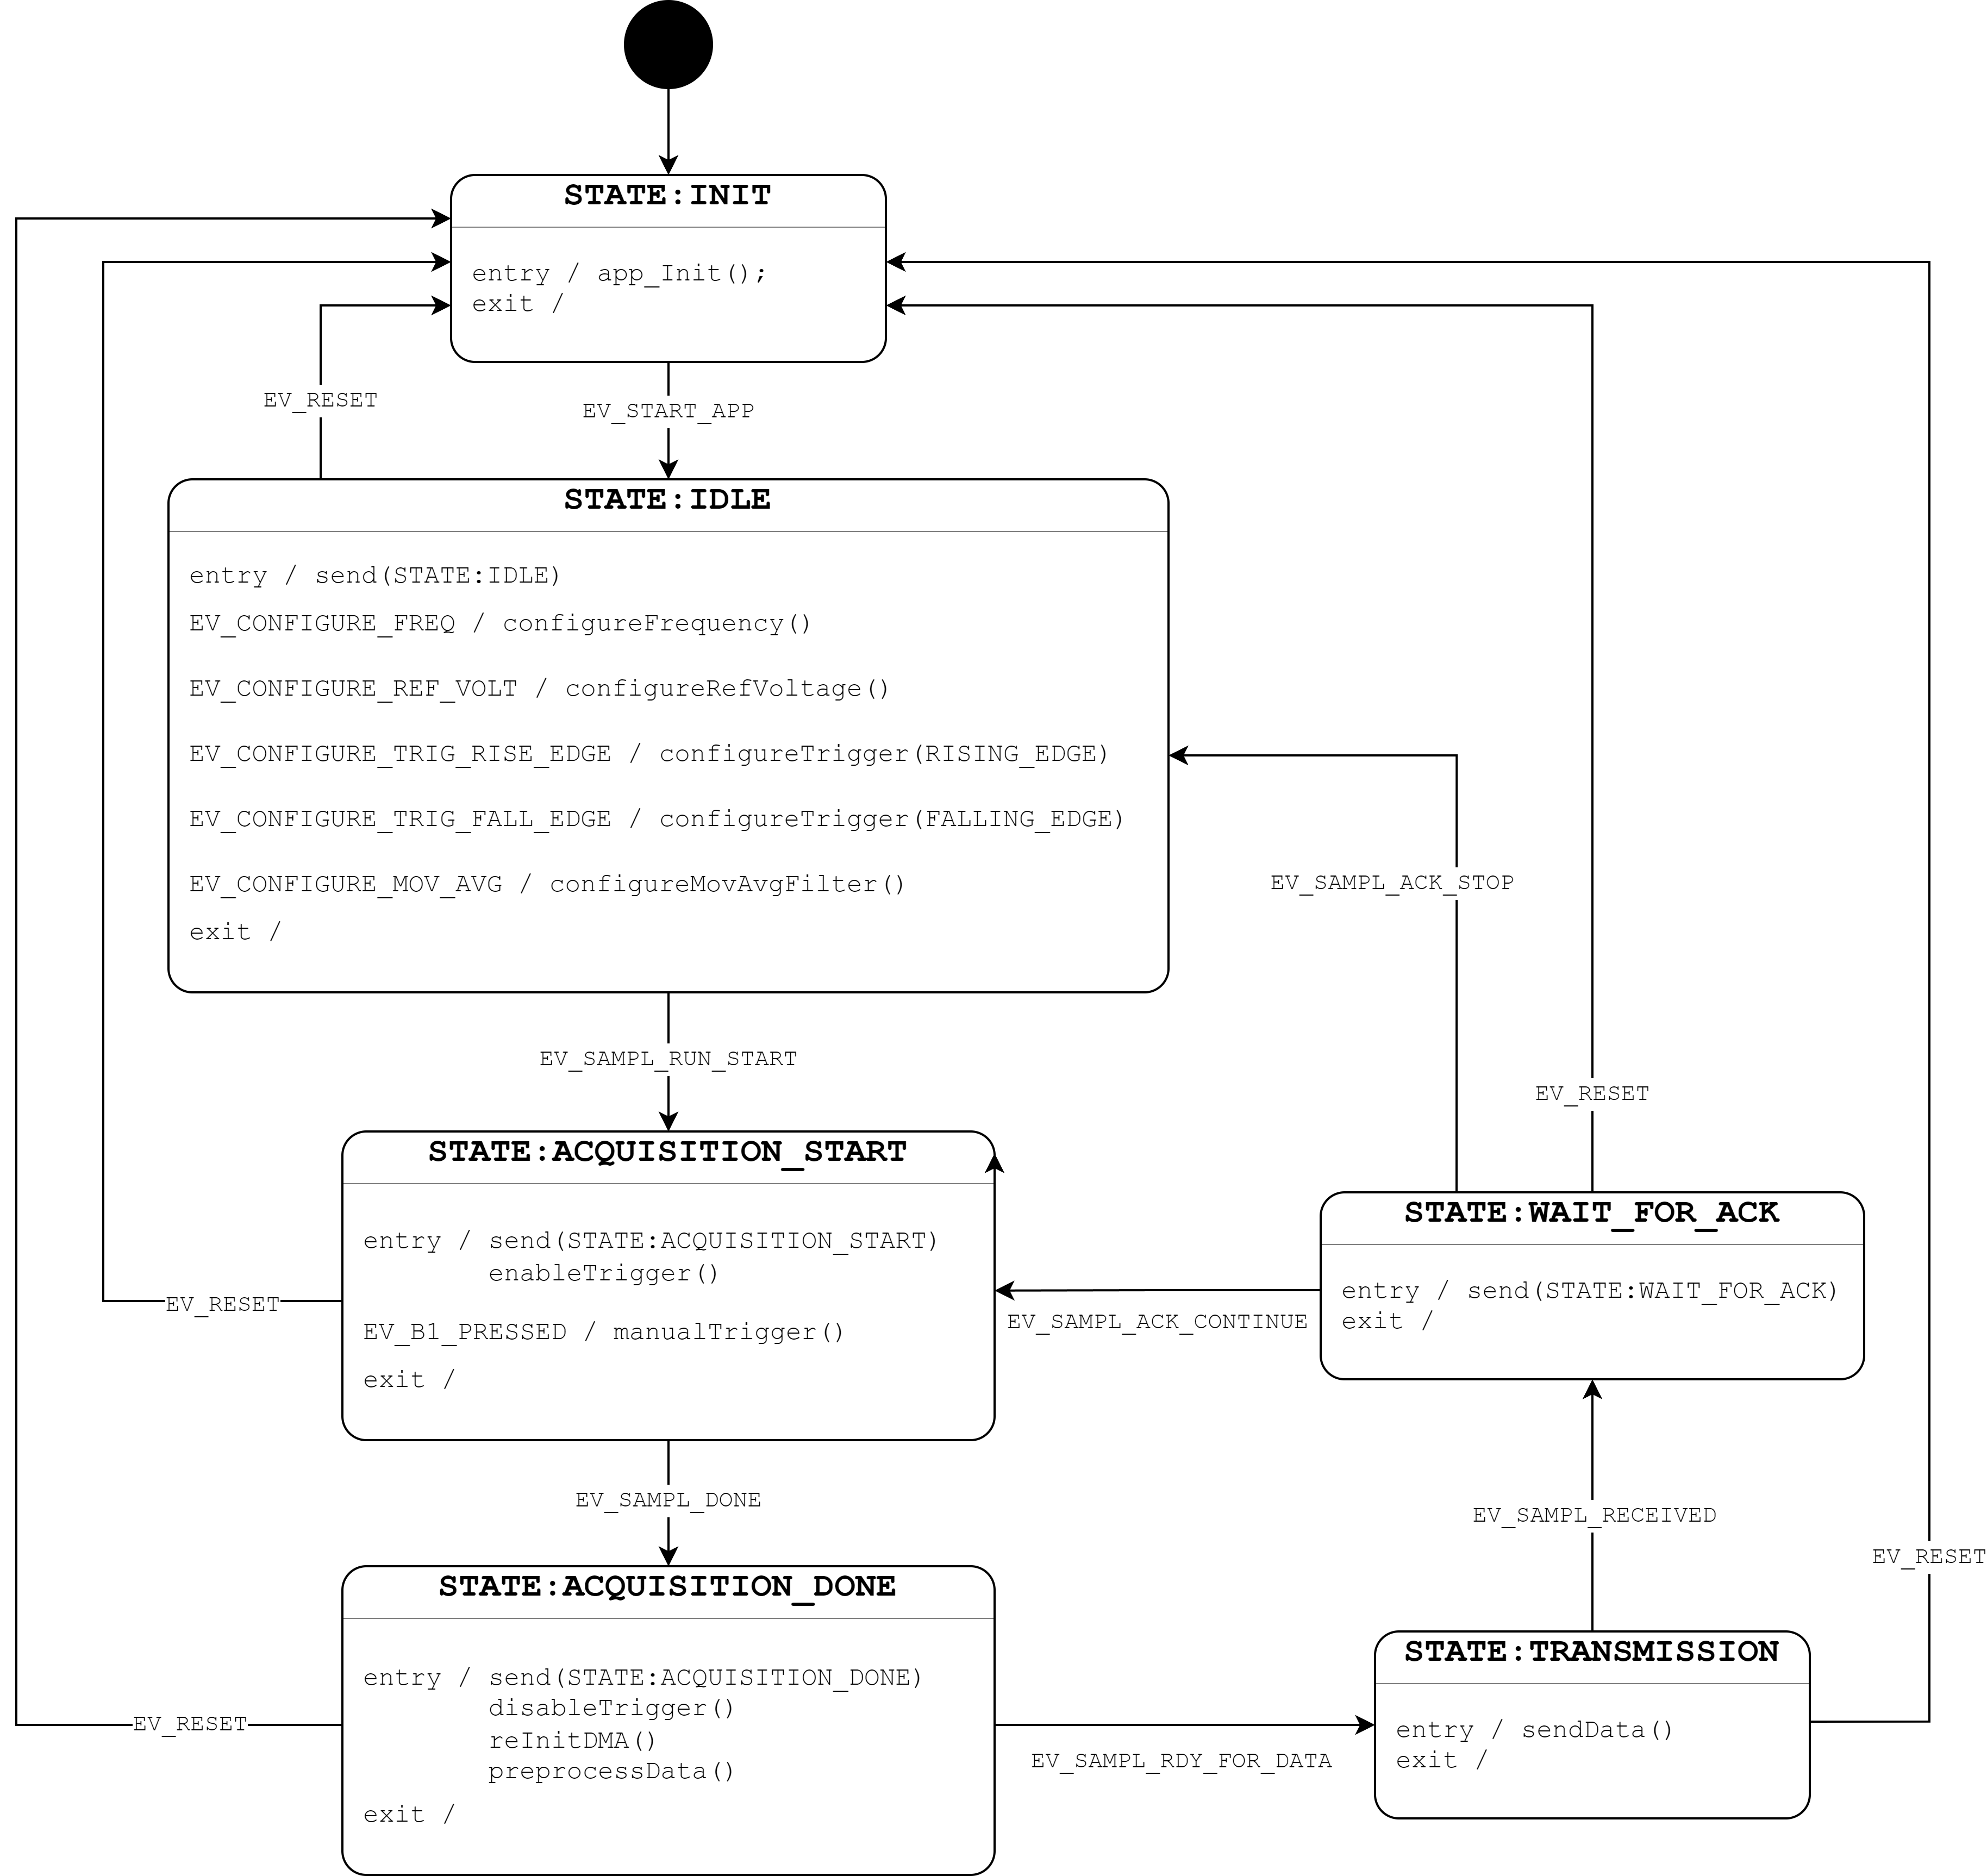
\includegraphics[scale=0.12]{StateDiagram_Firmware_V1.png} 
	\caption{Zustandsdiagramm für die Firmware}
	\label{fig:firmware_fsm}
\end{figure}

\underline{Event-Queue}\\
Die FSM verarbeitet Ereignisse über eine zentrale Event-Queue.
Dies erlaubt eine entkoppelte Kommunikation zwischen verschiedenen Modulen der Firmware und stellt sicher, dass Ereignisse nicht verloren gehen, auch wenn mehrere nahezu gleichzeitig auftreten.\\

Prinzipieller Ablauf:

\begin{enumerate}
	\item Ein Modul erkennt ein Ereignis (z. B. Button-Druck, DMA-Abschluss, USB-Befehl).
	\item Das Ereignis wird als Event-Code in die Queue geschrieben („enqueued“).
	\item Die Hauptschleife der Firmware liest fortlaufend Events aus der Queue („dequeued“) und leitet sie an die FSM weiter.
	\item Die FSM entscheidet anhand des aktuellen Zustands und des Event-Codes, wie reagiert wird und ob ein Zustandswechsel nötig ist.
\end{enumerate}

Vorteile dieses Ansatzes:

\begin{itemize}
	\item Asynchrones Verhalten wird klar handhabbar.
	\item Saubere Trennung zwischen Ereigniserzeugung und -verarbeitung.
	\item Erweiterbar für zukünftige Ereignisse, ohne die Hauptarchitektur zu ändern.
\end{itemize}

\underline{Zustandsübergänge}

Die wichtigsten Zustandsübergänge lassen sich wie folgt zusammenfassen:
\begin{itemize}
	\item \emph{Systemstart:}\\
	Init → Idle nach erfolgreicher Initialisierung.
	\item \emph{Start der Datenerfassung:}\\
	Idle → Acquisition Start nach Empfang des Startbefehls von der PC-Anwendung.
	\item \emph{Abschluss der Datenerfassung:}\\
	Acquisition Start → Acquisition Done nach Abschluss der DMA-Operation.
	\item \emph{Übertragung der Daten:}\\
	Acquisition Done → Data Transmission sobald PC signalisiert, dass er bereit ist.
	\item \emph{ACK-Verarbeitung:}
	\begin{itemize}
	\item Wait for ACK → Acquisition Start für weitere Messung.
	\item Wait for ACK → Idle für Beendigung der Erfassung.
	\end{itemize}
\end{itemize}
\pagebreak


\subsubsection{Preprocessing-Konzept}


\underline{Umrechnung 12bit signed (ADC) in 16bit signed}\\
Die Übertragung der Abtastwerte erfolgt in Einheiten von Halfwords (2 Byte). Da die Rohdaten des ADCs als 12-Bit signed Integer vorliegen, werden sie vor der Übertragung in einen gängigen Datentyp umgerechnet. Verwendet wird dabei ein 16-Bit signed Integer (\texttt{int16\_t} in C), da ein nativer 12-Bit Integer-Datentyp nicht existiert.\\
Durch diese Umwandlung können die Daten auf der PC-Seite direkt weiterverarbeitet werden, ohne dass zusätzliche komplexe Konvertierungsschritte erforderlich sind. Insbesondere kann die Empfangssoftware (Python-Anwendung) die empfangenen Werte unmittelbar als 16-Bit signed Integer interpretieren und anschließend in den gewünschten Zieldatentyp umwandeln. Ein weiterer Vorteil der Umrechnung liegt in der verbesserten internen Weiterverarbeitung auf Mikrocontroller-Seite. So konnten die Daten vor dem Versand beispielsweise effizient für die Anwendung eines gleitenden Mittelwertfilters aufbereitet werden (vgl. nächster Abschnitt).\\

Nachfolgend sind mögliche Algorithmen als Python-Code beschrieben:\\

\textbf{1. Sign-Extend (Shift-Methode)}
\begin{lstlisting}[language=Python, caption=Sign-extend (Arithmetisches Shift schiebt das MSB nach)]
def sign_extend_12_to_16(value12: int) -> int:
    # 12-Bit Zahl um 4 nach links, dann arithmetisch nach rechts
    return (value12 << 4) >> 4
\end{lstlisting}

\textbf{2. Zweierkomplement rückwärts: invertieren → +1}
\begin{lstlisting}[language=Python, caption=Zweierkomplement rückwärts aufgelöst.]
def twos_complement_backward_invert_plus1(value12: int) -> int:
	if value12 & 0x800:  # Vorzeichenbit pruefen
		inverted = (~value12) & 0xFFF  # Nur 12 Bits
		magnitude = inverted + 1
		return -magnitude
	else:
		return value12
\end{lstlisting}

\pagebreak

\textbf{3. Zweierkomplement rückwärts: -1 → invertieren}
\begin{lstlisting}[language=Python, caption=Alternative zu 2.: Erst -1 $\rightarrow$ dann invertieren.]
def twos_complement_backward_minus1_invert(value12: int) -> int:
	if value12 & 0x800:  # Vorzeichenbit pruefen
		decreased = (value12 - 1) & 0xFFF
		magnitude = (~decreased) & 0xFFF
		return -magnitude
	else:
		return value12
\end{lstlisting}

\underline{Gleitender Mittelwertfilter}\\
In \autoref{subsec:digital_filtering} wurden bereits die Grundlagen zur digitalen Filterung von Signalen geliefert. Diese wird in der Vorverarbeitung mittels \emph{gleitendem Mittelwertfilter} umgesetzt, welcher zufälliges Rauschen aus dem Signal herausfiltern kann. Dies ist insbesondere bei verrauschten Signalquellen mit kleiner Ausgangsamplitude interessant. Das Funktionsprinzip des Filters wurde bereits im oben genannten Grundlagenteil erläutert. Nachfolgend ist noch ein Pseudocode zu finden, der den Filteralgorithmus beschreibt (aus Signal Processing; \textbf{Quelle angeben}).\\

\textbf{Filteralgorithmus angeben!}
\pagebreak

\subsection{Implementierung}

\pagebreak

\subsection{FW-Test}

\pagebreak

\section{Schnittstelle Firmware - Software}

\subsection{Konzept der Kommunikation (USB CDC)}

\pagebreak

\section{Software (SW)}
\subsection{Entwurf}

\pagebreak
\subsection{Implementierung}

\pagebreak

\subsection{SW-Test}

\pagebreak

\section{Zusammenführung}
\subsection{Entwurf}
\subsection{Implementierung}
\subsection{SW-Test}

\pagebreak

%%%%%%%%%%% Schluss %%%%%%%%%

\pagebreak

%%%%%%%%%%% Ergebnisse %%%%%%%%%%%
\section{Ergebnisse}

\pagebreak

%%%%%%%%%%% Fazit und Ausblick %%%%%%%%%%%
\section{Fazit und Ausblick}

\pagebreak

%%%%%%%%%%% Literaturverzeichnis %%%%%%%%%%%
\section{Literaturverzeichnis}
\printbibliography
\pagebreak

%%%%%%%%%%% Abbildungsverzeichnis %%%%%%%%%%%
\section{Abbildungsverzeichnis}
\listoffigures
\pagebreak

%%%%%%%%%%% Abkürzungsverzeichnis %%%%%%%%%%%
%\section{Abkürungsverzeichnis}

%\begin{acronym}
%\acro{Abk.}{Abkürzung} % Im Text mit \ac{Abk.} verwenden
%\end{acronym}

%\pagebreak

%%%%%%%%%%% Anhang %%%%%%%%%%%
\appendix
\section{Anhang}
\label{sec:appendix_a}

  
\end{document}
